\documentclass{book}

\usepackage{graphicx}
\usepackage[space]{grffile}
\usepackage{latexsym}
\usepackage{textcomp}
\usepackage{longtable}
\usepackage{multirow,booktabs}
\usepackage{amsfonts,amsmath,amssymb}
\usepackage{natbib}
\usepackage{url}
\usepackage{hyperref}
\hypersetup{colorlinks=false,pdfborder={0 0 0}}
\usepackage{latexml}
\usepackage[utf8x]{inputenc}
\usepackage[english]{babel}

\usepackage{listings}

\begin{document}


\author{Radek Ježdík\\ Czech Technical University in Prague }


\title{Event Sourcing Design Pattern in a Java Enterprise Application}

\bibliographystyle{plain} 

\maketitle
 
\frontmatter 
\tableofcontents 
\newpage




\section{Introduction}\label{introduction}

In software engineering and development, there are many problems the
developers need to focus on to build a successful system. Many
difficulties come early in the design phase of the software and
developers had better have the knowledge and the proper tools to design
and build the software, so it is successful, bug-free, maintainable, and
usable. The trouble is that there is no single ``right way'', a silver
bullet, which can be used universally in software development because of
the complex nature of a domain that the projects usually solve. And of
course, even experienced software developers cannot possibly know every
problem the software can run into later in development.

However, a successful project --- that is a project built according to
customers' needs, in time, and on budget --- does not say anything about
the project internal code and design quality. The project, even if it
works as required, may be very brittle to change in its internals and
the code may be so complex that maintenance becomes very hard. This can
result in the introduction of bugs into the code that are, consequently,
difficult to find and fix. This situation usually happens in projects
that need to respond to changing requirements.

Some of the problems turned out to be so common that they needed to be
addressed in most of the projects, and so, over time, so-called patterns
and best practices formed to help solve the problems, or, at least,
diminish their effect. So, one of the best things software developers
can have is the knowledge of these patterns and best practices that were
already used and proven to work by someone else. This knowledge allows
them to tackle some of these common problems while making the code and
design easy to understand, maintain, change, and extend. This applies
not only after the project is done but also during the development of
the software itself, where numerous problems can emerge. Choices taken
prior to starting the development of some software, even if they were
thought through carefully, may not take into account problems that might
come during the development.

In recent years, there has been a notable shift in how applications are
run and built. More and more, applications are being moved from the
on-premise environments to the web. This has a number of advantages,
e.g.~the application can run on multiple devices, it supports instant
updates, the project can target a bigger audience, etc. Cloud computing
certainly had its part in the process. Inevitably, the situation brought
new problems into the web software development that the known patterns
did not address in that environment, e.g.~fine-grained scalability,
performance, changing requirements, multitenancy, multiuser
collaboration, etc. All this also affects how the applications are
structured and designed. If projects are expected to grow, the
applications that target the web must be prepared for the problems it
entails.

New patterns and practices evolved in the meantime to address the new
issues. Event sourcing and its companion Command Query Responsibility
Segregation (CQRS) are two examples which have been highly discussed in
articles and conferences in the last years. Their core ideas and
benefits are interesting enough to aim the attention at their details
and implementation. And since Java is one of the most used programming
languages in the enterprise software development \cite{java}, it is
appropriate to study and apply the patterns using this language.

\subsection{Goals}\label{goals}

The goal of this diploma thesis and the work behind it was to study the
basic principles of the Event Sourcing and Command Query Responsibility
Segregation patterns and to implement them into a real-world software
project written in the Java programming language. Additionally, it aimed
at comparing the design patterns with the traditional architecture of
enterprise applications.

\subsection{About the text}\label{about-the-text}

The following chapters explain the basic ideas, benefits, and
disadvantages of the patterns, and describe the path taken in
implementing the patterns into an existing software project written in
Java --- Integration Portal --- in which the benefits over the original
design are practically examined.

The first part of the thesis describes the idea of Event Sourcing and
the Command Query Responsibility Segregation design pattern, which is
usually implemented in tandem with Event Sourcing. The second part
introduces the Integration Portal project and its original design that
was, as part of this diploma thesis, subjected to refactoring into Event
Sourcing and CQRS design. Finally, the whole process and the experience
are described together with a discussion of the issues that were
introduced by the refactoring and suggestions of how they could be
handled.

In conclusion, this thesis should provide enough necessary information
to obtain a basic understanding of Event Sourcing and CQRS and describe
the advantages and disadvantages of this design, both in general and in
Java implementation.


\section{Event Sourcing and CQRS Design
Patterns}\label{event-sourcing-and-cqrs-design-patterns}

In this chapter, the core ideas of Event Sourcing and Command Query
Responsibility Segregation design patterns are described. The basic
principles and terms of these patterns are presented to the reader so
they acquire enough information to understand the next chapters.

\subsection{Introduction}\label{introduction}

The traditional software described in most books and online tutorials
usually stores its current state in a structural model that is persisted
to some kind of a database system, e.g.~a relational database. The
principles of event sourcing, that will be described further in the
text, puts the idea of such current state aside. Together with the
Command Query Responsibility Segregation design pattern, they have a
number of interesting effects on application development and design, and
may contribute to increasing the business value of an application. More
information about the benefits will be covered in the following
sections.

It's appropriate to say that neither of the two patterns implies the
other; they can work independently. However, they nicely complement each
other to form a very effective and powerful design for a system.

Both design patterns were popularized by the practitioners of the
Domain-Driven Design (DDD) \cite{ddd} methodology for software
development. And so, the DDD concepts and ideas influenced the
implementation details of the two patterns. DDD is a very comprehensive
subject on its own and as such will not be discussed in this thesis
apart from the terms and principles that are involved in the presented
patterns.


\subsection{Event Sourcing}\label{event-sourcing}

The following text describes the Event Sourcing (ES) pattern in detail.
First, to help understand the idea of the pattern, some necessary
definitions are presented. Finally, a few reasons why use Event Sourcing
are discussed with some examples of where ES is an advantage for
applications.

Event Sourcing is a way of persisting the state of an application by
storing the history that shaped the application's current state. Instead
of storing only the current state in some fixed structural model,
e.g.~in a relational database, event-sourced model stores a list of
events that happened in the system in its entire lifetime.
\cite{journey} \cite{greg-youtube}

\subsubsection{Domain event}\label{domain-event}

The core term in Event Sourcing is a domain event, which is usually
referred to as just an event. A domain event is a fact about an
application state transition. In other words, it describes something
that has happened to the system and resulted in some state change.

In most cases, there are a number of different kinds of events in the
system, each describing a different type of the change. For example,
``\emph{product added to user's cart}'' or ``\emph{product reserved}''
events could fit in some online shopping application. Events have a
single source that publishes the event (publisher) and one or more
receivers that process the event.

Because events describe something that has already happened, they are
immutable --- they cannot be changed or undone in the very same way we
can't change our past in the real world. But there can be subsequent
events that can alter or cancel the effects of the previous events, e.g.
``\emph{reservation canceled}''.

Event names should also reflect their intents from a business point of
view. The ``\emph{address corrected}'' and ``\emph{customer moved}''
events reflect different business values in the domain, even though they
would probably result in the same data change (updating the address).

As you've probably noticed, the events should be named in the form of a
verb in the past tense. That is because the domain event symbolizes
something that has already happened, a historic event that marks a state
transition in the application.

\subsubsection{Event log}\label{event-log}

How events get generated will be described in the section about the CQRS
design pattern. First, let's take a closer look at storing the events.
As already mentioned, the events are saved to persistent storage in a
representation called the event log, a list of events in the same order
they have actually occurred in the system. Not only that, the event log
is append-only, which means new events can only be added to the end of
the log. This rule, together with the immutability of events, means that
the already persisted list of events can never be changed or altered ---
no inserting, editing, or
deleting.\footnote{This is true conceptually, but in some cases, e.g. for legal reasons, the events can be changed or deleted.\cite{greg-youtube}}

The actual storage mechanism is not very important and it can differ in
implementation --- it can be an in-memory list (best suited for
testing), a file system, a relational database, or a storage
specifically designed to persist a lot of messages in large quantities
with great performance. It depends on the requirements and use cases to
choose the best strategy for persisting events.

The event log is then used to recreate the current state of the
application (or its parts). The exact way that this is carried out will
be described in detail in the section about CQRS.

\subsubsection{Rationale}\label{rationale}

The general idea of Event Sourcing has been used for ages but not so
much in typical software development. As stated previously, most of the
applications use the concept of current state that is usually persisted
in, for example, a relational database. That is the reason why most
developers tend to think about the state in a structural sense such as
in Figure~\ref{fig:relational-model}. In an online shopping application,
for instance, a model of a purchase order could look like that.


\begin{figure}[h!]
\begin{center}
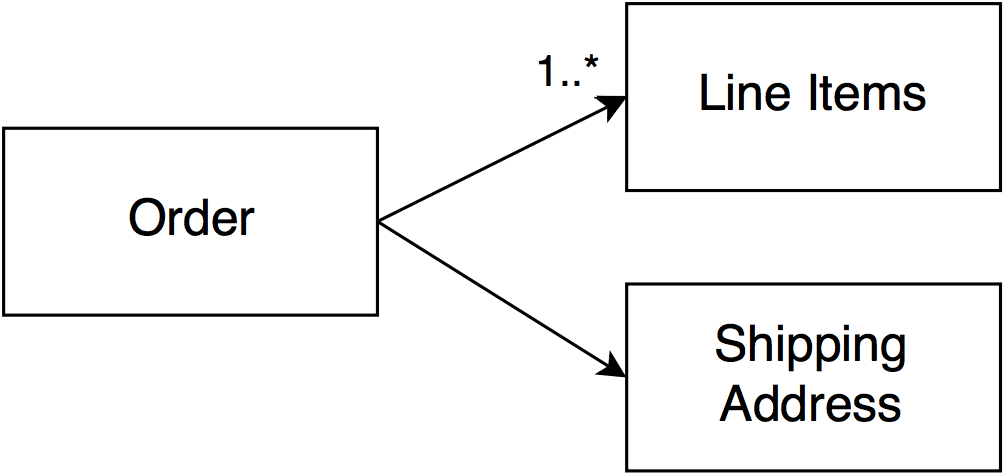
\includegraphics[width=0.7\columnwidth]{figures/relational-model/relational-model}
\caption{An example of a structural model of a purchase order%
}
\end{center}
\end{figure}

However, this is not the only conceptual model that can represent an
order. Other solutions offer different properties that suit other use
cases better. For example, a relational database is not very suitable
for full-text indexing and searching. Other systems would benefit more
if they used a graph database for some part of the application instead.
The point is that there is no single model that could be used
universally for every possible case that the system needs to address.
Moreover, the structure of the application data tends to change over
time.

In an event-sourced model, the structure of the current state is
irrelevant. To make the explanation clear, let's take an example from
bookkeeping or bank accounts where everything is stored as a list of
accounting entries, or entries of money deposits and withdrawals. When
you receive your bank statement, you can see that it's presented as a
list of entries specifying what happened to your account each time a
transaction happened and how much money was involved in each
transaction. If you take all these entries and sum them up (positive
values for deposits, and negative for withdrawals) you get your total
account balance. This is how banks worked and are still working --- they
keep all these entries as a history of account transactions and by
summing them, they calculate the account balance.

However, by keeping only the current state (balance of a bank account),
a lot of valuable historic data is lost, e.g.~the information about the
time a state change happened, who invoked the change, and so on. This
historic data may remind you of something called an audit log.

An audit log is the very same thing as the bank statement from the
accounting example. It is effectively a log of events that happened to
the account throughout its entire existence. System administrators may
use the audit log to learn who did what in the system and track the
corresponding changes. Many systems actually need an audit log (banking
systems by their nature do) for the purpose of regulation or auditing.

In many systems, an audit log is a separate module that is updated by
the code handling the state changes. However, this way may be
error-prone as developers who make changes to the code must be very
disciplined and remember to update the audit log to store the correct
event in the log. As the system grows bigger, it may take a lot of
effort to maintain the audit log, and, more importantly, prove it is
correct!

Event Sourcing takes the opposite approach. It makes the audit log the
core concept for system state transitioning. That means the source for a
system's state is the audit log, a list of events, in the first place.
From this log the current state of the application can be computed, much
like the account balance is computed from the list of account entries.
For example, see the Figure~\ref{fig:events}. This computed value would
be called a projection. It may be viewed as a function of a list of
events which returns a projection of those events.


\begin{figure}[h!]
\begin{center}
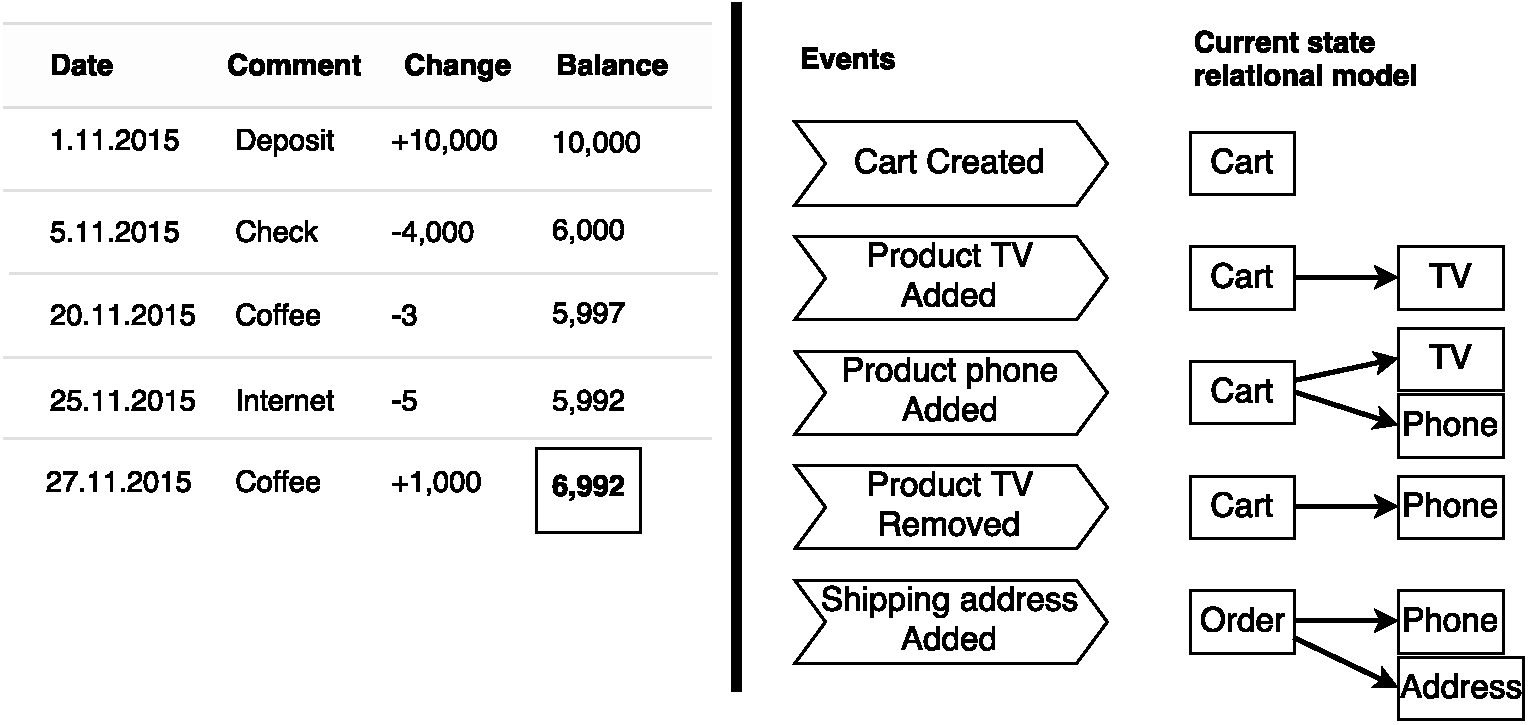
\includegraphics[width=0.98\columnwidth]{figures/events/events}
\caption{Two examples of event projections. On the left, an accounting example
with total balance being updated with each transaction. On the right,
there is a list of events in an online shopping application that builds
the relational model.%
}
\end{center}
\end{figure}

The advantage of this design is that we can compute many variations of
projections to suit our needs --- we can populate the application state
in a relational database, or create a search index for our data, etc.
Since we store all events that happened in the system in our audit log,
we can add a new projection at any time by simply processing all the
historic events through a system that generates the new projection.
Conceptual process flow of that processing is shown in Figure~\ref{fig:projections}.

Another example of a real-world event-sourced model can be found in many
relational database engines. An interesting aspect of these database
systems is that, internally, they usually keep some kind of a
transaction log where they store all the changes that were applied to
the database \cite{cqrsnu-eventsourcing}. This log is then used, for
example, to handle database transactions, crash recovery, and
replication. It is very easy to replicate data if they are represented
as immutable events in an append-only, sequential log. To replicate, a
node just needs to send the events that are new since the last
replication and the receiving node applies these changes to itself,
making both nodes synchronized \cite{replica}.

In summary, instead of storing the current state of the application,
Event Sourcing primarily stores facts about changes (events) that
happened to the application. The current state is degraded to be
transient, meaning that we can throw it away and build it again just by
processing events one by one. The benefits of this design are that we
automatically get a correct audit log (in some cases required by the
law), and a way to build the current state by making projections of the
events. But there are other beneficial use cases, that would not be so
straightforward or possible at all without it. The next paragraphs
describe some of these cases for the reader to consider.


\paragraph{Rebuilding the read model}\label{rebuilding-the-read-model}

As stated above, there is more than one way how to model and structure
application data. Some models are good for some tasks than the others.
More importantly, the models tend to change over time to, for example,
accommodate new requirements. Event sourcing enables us to change models
or create new ones from the events by making projections. This can be,
for example, a model used by an application to query data to be
presented to users (a so-called read model). On top of that, it allows
us to rebuild the model to a different structure. We can change the way
the user sees the data by projecting the events again but structuring
the model differently. We can also use the existing events to build a
separate read model that will exist next to the original one. For
instance, a search index of the application data, which is stored in a
full-text-search server instead of a relational database, can be better
in searching capabilities. The process of updating or rebuilding the the
read models is shown in Figure~\ref{fig:projections}.


\begin{figure}[h!]
\begin{center}
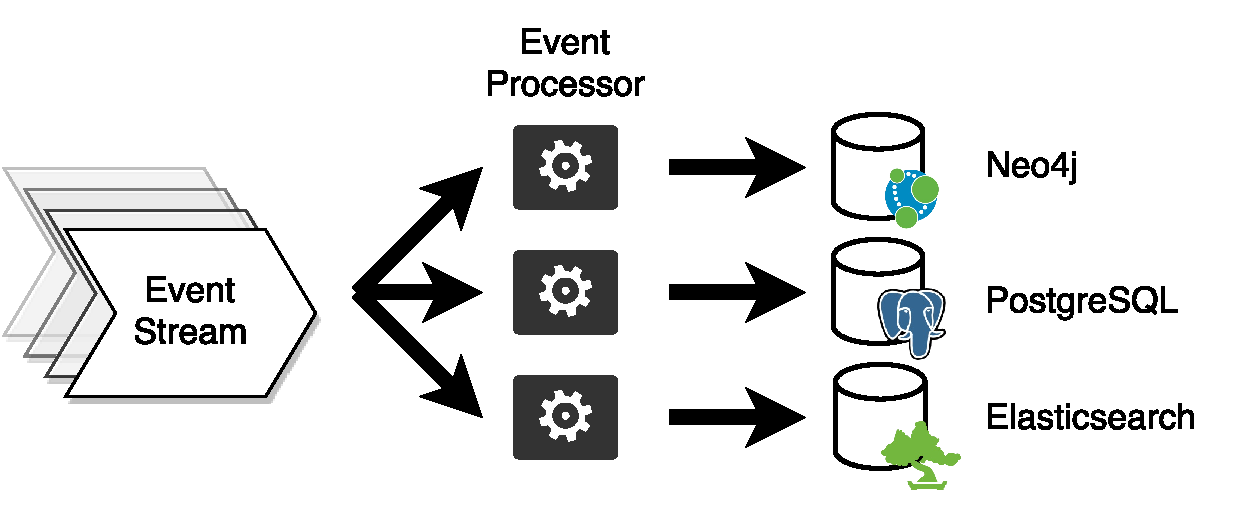
\includegraphics[width=0.84\columnwidth]{figures/projections/projections}
\caption{Updating (or rebuilding) read models from events%
}
\end{center}
\end{figure}

\paragraph{Fallback after a failure}\label{fallback-after-a-failure}

When deploying a new version of an application into production for our
users, in many cases, it also means that we need to update the RDBMS
tables with a new schema and/or update the data. Imagine that after such
deployment the system works for only a week before it crashes because of
some serious failure. If fixing the system requires a lot of time it is
probably best to fall back to the last working version.

If we use version control systems or other tools to back up the code
base it is possible to recover the working code easily. Getting back the
database state, however, may be impossible because of the destructive
changes made to the production database during deployment. The original
data for the old version may be lost forever because of the schema
update. If the database was backed up before the deployment we can get
the original database back. However, we would lose all the data the
users created during the week that the new version was working.

With Event Sourcing, this fallback can be accomplished easily. Since
events must never be altered, we still have all the necessary data to
recreate the original data model by replaying all the events including
those created in that week.

But we can go a step further in our deployment process and keep the two
systems, the original version, and the new version, running side by
side. After deployment, the new version can take control of generating
the events, while both versions can process them individually into their
own data models in separate databases. If anything goes wrong with the
live version, we can just switch back to the original (but still
up-to-date) version running in parallel. This way the users will not be
affected by long-lasting down times leaving we more time to fix the
problem.

\paragraph{Event processing}\label{event-processing}

With a complete event log, we can make projections of the data for the
users. But we can also create other systems around the same event log.
The systems can then use some or all the events to do tasks like:

\begin{itemize}
\tightlist
\item
  \textbf{monitoring} -- for the purpose of statistics regarding, for
  example, exceptional behavior (e.g.~frequency of events or unexpected
  order of events).
\item
  \textbf{fraud detection} -- if a state, which is considered a fraud by
  some specified rules, is reached, the processor can notify interested
  people to act upon the situation.
\item
  \textbf{data analysis} -- for inspecting the events to get some
  information valuable for the business, e.g.~what action is done the
  most by the users at what time of a day.
\item
  \textbf{data mining} -- to find some new trends and correlations in
  the data.
\item
  \textbf{system integration} -- to merely convey messages and data
  between multiple systems.
\end{itemize}

\paragraph{Deriving business value from the event
log}\label{deriving-business-value-from-the-event-log}

Event Sourcing can help fulfill new business requirements that involve
old data easily. Imagine that the project stakeholders come up with a
new requirement for an already working online shopping system. The
feature they want to implement is a suggestion mechanism that shows the
users the products they removed from their cart just before checking
out. Possibly, the users wanted to buy these products but they removed
them from the cart because the total order price was too high. The users
may want to buy the products next month, though. To suggest those
products to the user on their next visit we need the information that
the products were removed from the cart just before checkout. If we
designed our domain events properly we should have that information for
every user in the system already stored as events in the event log. We
can build this feature easily using the old events and suggest the right
products to each user immediately after the feature deployment. This is
a very nice advantage over the systems that store only the current state
because these systems do not have the data beforehand. The system
wouldn't be able to suggest anything until the next user removes a
product from their cart.

A very similar example of a requirement that involves historic data is a
chart of price development for a product over time. Many online shopping
systems present this kind of chart to their users. It is not possible to
(immediately) accomplish this requirement in an application that stores
only the current state (the current price of the product). In an event
sourced system, this task is easy to accomplish as we probably already
have all the events with the price updates for every product.

\paragraph{Debugging}\label{debugging}

We can use the event log to examine a fault in our system. Imagine that
a user reports a bug without specifying the steps to reproduce the bug.
This is usually a nightmare for software developers isolating the bug.
But with Event Sourcing, we have the whole history of events applied to
the application and stored in a log. Thus, we can go back in time by
replaying the events (similar to model rebuilding) and see what the user
did, by looking at the events, at the exact time the bug happened. We
can then use standard debugging tools to see what code got executed by
the application and why it resulted in producing the bug.

Compare this feature with traditional logging. Logging is a way of
saving events about the system execution in a textual, human-readable
format to understand the activity of the system and to diagnose
problems. However, this format is not very helpful if the log messages
are not comprehensive enough, which is completely in the hands of the
developers. Also, it is less convenient to restore the system state from
these messages because they are, unlike in Event Sourcing, disconnected
from the code execution.

\paragraph{Testing}\label{testing}

\textbf{TODO}

\subsubsection{Summary}\label{summary}

As you can see, Event Sourcing isn't a complicated idea at all. The
premise is that we don't primarily save the current data of an
application state, but we instead save all the events that represent the
state changes in the system in a persistent log. We then use this log as
the \emph{single source of truth} to determine the actual state of the
application for various cases.

The concept, however, doesn't inherently say anything about how to get
the state or how to see current data of an application. This is a job
for the design pattern called CQRS, described in the next section.


\subsection{Command Query Responsibility
Segregation}\label{command-query-responsibility-segregation}

This section is intended to provide information about Command Query
Responsibility Segregation, the problems it aims to solve, and its
connection to Event Sourcing.

The foundation for the CQRS pattern is the idea that the system making
writes and reads using the same data model is discouraged and dividing
these responsibilities both simplifies the design and easily enables
horizontal scaling and increases performance. It extends the idea of the
CQS (Command Query Separation) principle for designing interfaces of
objects. CQS says that the object's methods should be either commands or
queries. The responsibility of a query is solely to return data and not
to alter the state of the object. On the other hand, a command should
only change the state of the object but never return any data
\cite{journey}.

CQRS takes this idea and applies it to the system level where it
strictly separates the responsibility for handling a command input (to
change the application state) from the responsibility of
side-effect-free reading of application data \cite{journey}. You can see
the conceptual view of the CQRS design in Figure~\ref{fig:cqrs-concept}.


\begin{figure}[h!]
\begin{center}
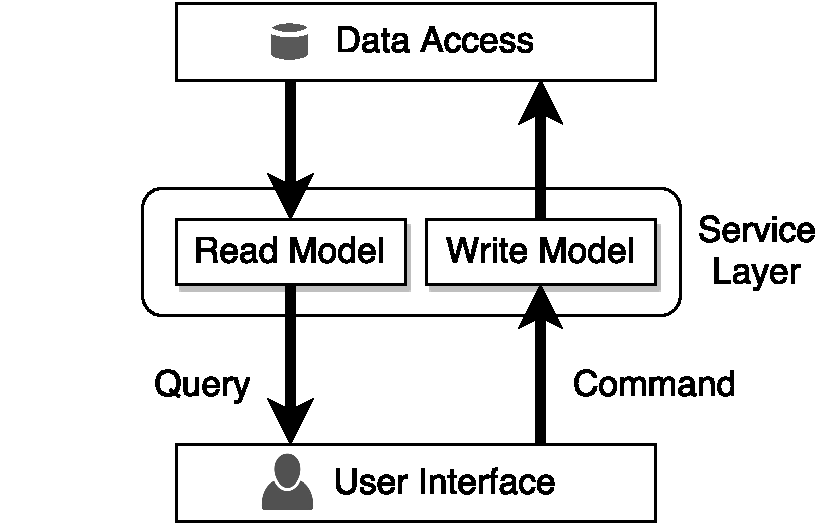
\includegraphics[width=0.49\columnwidth]{figures/cqrs-concept/cqrs-concept}
\caption{Concept of Command Query Responsibility Segregation%
}
\end{center}
\end{figure}

If each of the two concerns is separated to a different module, it
provides us some benefits described in the following paragraphs.

\subsubsection{Rationale}\label{rationale}

There are few reasons to consider splitting the two responsibilities.
First is that reading the application data (querying) is not something
that usually needs transactional invariants to be involved; that is
something commands need to address. A query just returns data. On top of
that, queried data are usually represented in the form of screens (or,
based on your use cases, other types of an interface) that the users are
presented with, so the perception of queried data on a screen can be
different than the model used to alter the data. This model, sometimes
called a write model, must uphold transactional invariants or business
rules of domain entities and it is usually subject to concurrent changes
and/or multi-user collaboration.

The second, more important thing is that usually it is the read side of
your application that needs to be scaled to ensure the quality of your
system for a bigger audience. In many systems, a ratio of reads to
writes can be several orders of magnitude \cite{cap}. Instead of scaling
everything in the system it is better to focus on the part of the
application that is most heavily used, i.e.~the read side.

This leads us to an interesting aspect of most queries and that is
relaxed consistency. In round-trip based web applications, users already
interact with stale data in their browsers. Imagine the time that a
response takes to return from a server to a user and the time the user
spends viewing the screen before making interaction. At any point, the
data could have been mutated on the server by other users or the system
itself and so, the user sees data that is inconsistent with the server.
So, relaxing the consistency of queried data, so it can be easily
scaled, is not a big issue. The important thing to mention here is that
relaxing the consistency does not mean that the data is inconsistent on
the read side. It is rather \textbf{eventually consistent}; that means
that correct and consistent data is returned by the query at some point,
but it just may not be immediate. The delay before the read side is
updated is not something that would break the system in most cases.

This, however, does not apply to the write side where it is necessary to
always operate on the current state to reliably ensure full consistency.
This means that the write side is usually a lot harder to scale and to
ensure being consistent at the same time. But, depending on the type of
your system, scaling the write side is not always needed.

As a final note on reasons for using CQRS, let's mention that it enables
the application to easily have different types of read models running in
parallel. In many cases, the application needs to query its data from
different types of data models to function well. As an example, a
full-text search is not something very efficient to do in a relational
database. The same applies when querying data that are structured as
graphs. A single model that does everything right does not exist; some
models do things better than others in specific circumstances. CQRS
together with Event Sourcing enables us to create multiple read models
of different types very easily.

\subsubsection{Terminology}\label{terminology}

Before we get into implementing CQRS and Event Sourcing in Java it is
necessary to explain some of the terminology used in the process. In
\cite{journey}, the CQRS pattern was presented as hugely influenced by
the approach to developing software systems known as the Domain-Driven
Design methodology (DDD). The DDD approach describes a set of techniques
to analyze the domain of the system and to construct a conceptual model
from the results of that analysis. This model is then used for designing
large and complex domains and helps you solve the problems in the
domains.

However, it is essential to say that DDD does not dictate the usage of
CQRS, nor CQRS needs DDD for it to be implemented in the system.
However, in much of the existing literature these two principles are
used together and many CQRS practitioners use the terminology of DDD
\cite{journey}.

Because of that, let us succinctly describe some of the DDD concepts and
terminology that are usually involved in the CQRS pattern in the
following paragraphs. Relations of the terms in a complex system is
shown in Figure~\ref{fig:ddd}. You can find more information about DDD
in \cite{ddd}.


\begin{figure}[h!]
\begin{center}
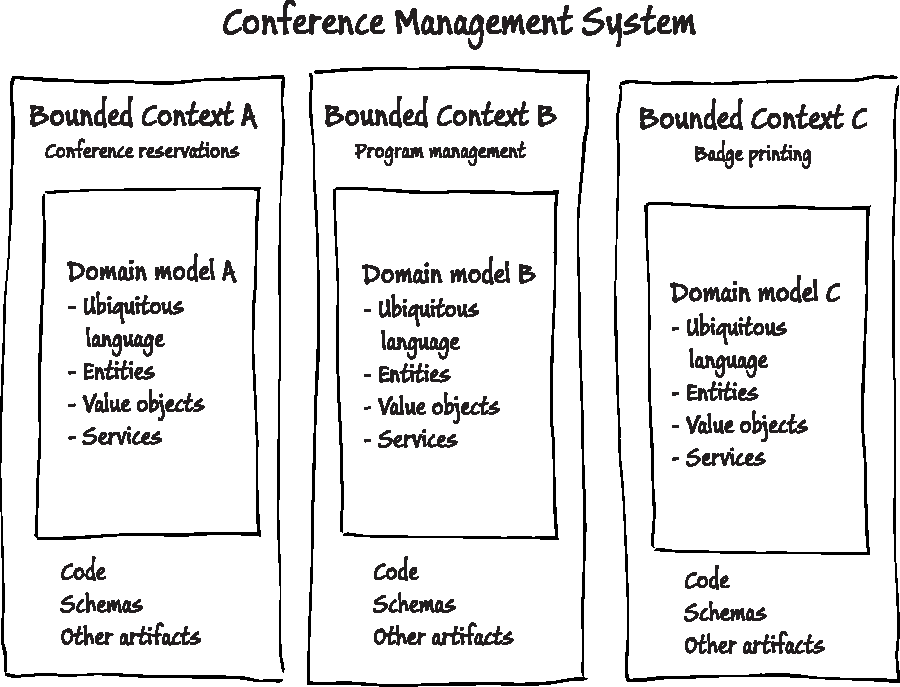
\includegraphics[width=0.7\columnwidth]{figures/ddd/ddd}
\caption{An example of relations between DDD concepts in a complex system. Source
\cite{journey}.%
}
\end{center}
\end{figure}

\paragraph{Domain model}\label{domain-model}

The core concept of DDD is the domain model. This model is built by the
domain experts and software developers who both form the team
responsible for developing the system. The model is used to capture all
of the relevant domain knowledge and to determine the scope and verify
the consistency of that knowledge. The domain is expressed in code and
is constantly maintained to reflect the changes as they occur in the
evolution of the domain knowledge.

DDD is focused primarily on the domain because that is where the value
of the software lies from the business point of view. The role of the
domain model is to capture what is valuable and unique to the business.
Domain models are typically composed of entities, value objects,
aggregates, and described using terms from a ubiquitous language.

\paragraph{Ubiquitous language}\label{ubiquitous-language}

Many problems in real-world software development arise from different
language nuances used by the software developers and the non-technical
domain experts when they communicate to each other. The concept of
ubiquitous language aims to create a dictionary that is strictly used
when talking or writing about the domain. If both parties use the same
language to talk about and to codify the domain to the domain model, the
risk of confusion or misunderstanding is reduced. DDD also leverages
that software developers are not just coding monkeys and they should
participate in constructing the domain model together with the domain
experts.

\paragraph{Entities and value objects}\label{entities-and-value-objects}

Two of the main building blocks that make up the domain model are
entities and value objects. \textbf{Entities} are objects that have
their own identity that continues through time. Entities may have
attributes that can change over time, but their identity stays unique in
the system (for example an application user). On the other hand,
\textbf{value objects} are defined by the values of their attributes and
not by their identity. For example, a customer's address is made up of
street, city, state, and so on, but for the purpose of that domain, it's
not necessary to make that address an entity with a unique identity.
Rather the values of the given attributes are what is important for
value objects. Usually, value objects are immutable, and if its
attribute is to change the value object is replaced with a new instance.
The difference from entities is that two entities might be equivalent in
all their attributes, but will still be distinct; in the case of value
objects, they would be considered equal.

\paragraph{Aggregates}\label{aggregates}

An aggregate is a unit of a transaction boundary. In DDD terms, it is a
cluster of related entities and value objects that are supposed to
remain consistent within the system. The lifetimes of its components are
bounded by the lifetime of the entire aggregate. An aggregate is
responsible for consistency and upholding the invariants (business
rules) that are set on its components by the domain. Also, aggregates
should not hold references to other aggregates as they should not reach
outside their consistency boundaries.

\paragraph{Aggregate roots}\label{aggregate-roots}

Since the aggregate is effectively a tree or a graph of objects, an
aggregate root is the object at the top. The aggregate root is
responsible for communication with and delegation to its child objects
and thus, it is the only entry point to the aggregate's objects from the
outside world. The assertion of invariants (business rules) is also its
responsibility.

\paragraph{Bounded context}\label{bounded-context}

All of the terms described above are used to create, maintain, and
manage a domain model. Using a single domain model for large systems may
be impractical, reducing consistency and comprehension. So, DDD adopts a
concept of bounded context. A bounded context is a context for a single
domain model. This allows us to create multiple small domain models,
each focusing on some group of functionality of the whole system.

\subsubsection{The CQRS concepts}\label{the-cqrs-concepts}

Now that the necessary terminology of Domain-Driven Design was settled,
let's introduce terms that are more related to CQRS concepts. Please
note that even though DDD and CQRS are not implying one another they are
usually used together in most of the literature. Thus, the distinction
of what is part of DDD and what is part of CQRS sometimes blends
uncertainly. Moreover, CQRS is to a greater degree a principle rather
than a design pattern with its own terminology. However, the CQRS
implementation established by using the domain-driven design comes with
a new vocabulary. Some of the terms described below can be used to talk
about DDD too and vice versa \cite{ddd-terms}.

\paragraph{Commands}\label{commands}

A command in CQRS is a way of expressing user's intent for the system to
do some action. The \emph{user} of the system can be a real person in
front of a screen or an external automated system. Both can send
commands to the system to perform some task. For example, ``\emph{Add
product X to cart Y}'' or ``\emph{Checkout}''. A command should clearly
reflect its intent because some command's intent may have different
invariant value than other commands. Thus, it's not very wise to create
a simple ``\emph{Update}'' command capable of updating anything, because
it does not capture the intent of the update. This leads us to the term
\emph{task-based user interface} which is described further below.

\paragraph{Command Handlers}\label{command-handlers}

A command is usually processed by a single recipient called a command
handler. The responsibility of the command handler is to execute code to
perform the action or task intended by that command. In a domain-driven
application, the command handler should validate that the command is a
valid command, then it should locate the aggregate instance that is the
target of the command (or create a new aggregate if that's the command's
intention) and call the appropriate method on the aggregate instance
with parameters from the command. Finally, it persists the new state of
the aggregate to storage.

\paragraph{Events}\label{events}

Events in CQRS are part of the messaging pattern and are a superset of
domain events. With that in mind, we can use these events for
communication and integration, whether that be between aggregates in the
same or other bounded contexts or with other systems or subsystems. They
have a special meaning for Event Sourcing which will be described later.
Events are published to subscribers that process the information that
something has happened in the system.

\paragraph{Event Handlers}\label{event-handlers}

Events are published to multiple recipients called event handlers. Event
handlers are subscribed for a particular type of event that the
subscriber knows how to handle. Their job is to receive an event, get
the target aggregate and call its appropriate method. Finally, it should
persist the new state of the aggregate to storage. Some event handlers
do not operate on aggregates at all and are used for \emph{messaging}
instead.

\paragraph{Messaging}\label{messaging}

Both \emph{commands} and \emph{events} implement the messaging pattern
that enables us to make a system driven by events (event-driven design).
This pattern provides us with a lot of flexibility because the messages
(commands and events) can be examined, prioritized, queued, partitioned,
subscribed to, retried, forwarded and so on. In CQRS, events can be sent
using some messaging protocol to other applications or subsystems in
order to, for example, update the read model. On the other hand,
commands can be prioritized or queued before they are actually sent to a
command handler. This, of course, depends on the requirements for the
system being developed.

\paragraph{Sagas and process managers}\label{sagas-and-process-managers}

Saga and process manager are often used interchangeably when referring
to a Process Manager. Both are strategies to handle long running
business transactions without using distributed transactions. Often
there is a situation where we need to coordinate communication between
multiple aggregates. Take an order process for example, when an order is
placed we need to wait for the user to pay, meanwhile, the products are
reserved for the user. At the same time, the order can be limited by
time and can be rejected if the user doesn't pay within some time
period. So a process manager acts as a mediator between the aggregates
conveying messages based on rules given by the process it manages.
Usually, it holds some internal state by which it decides to send new
events or commands to aggregates. An example of process flow of a saga
is shown in Figure~\ref{fig:saga}.


\begin{figure}[h!]
\begin{center}
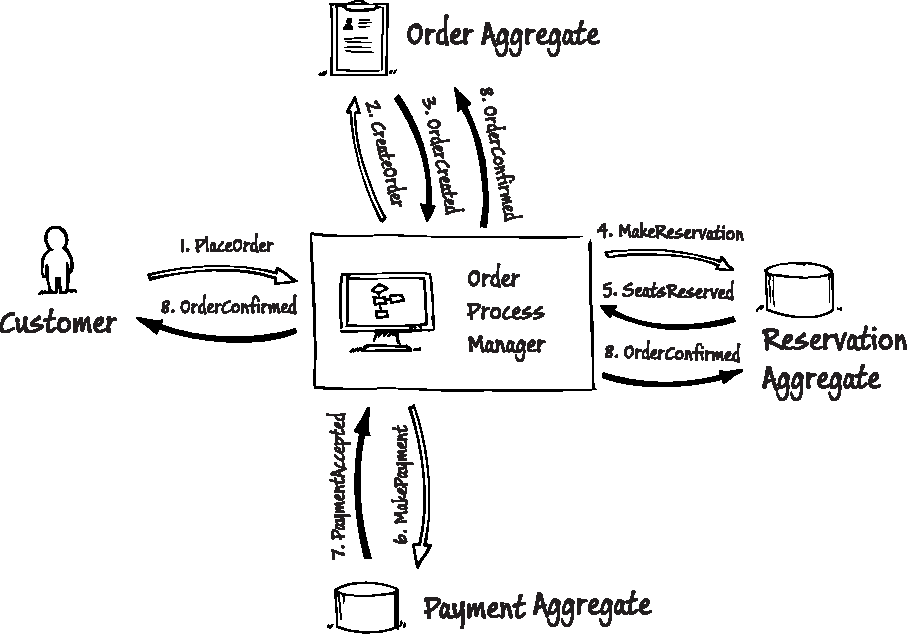
\includegraphics[width=0.7\columnwidth]{figures/saga/saga}
\caption{Simple process manager that tracks the state of an order of seats at a
conference. Source \cite{journey}.%
}
\end{center}
\end{figure}

\paragraph{Task-based user interface}\label{task-based-user-interface}

In a typical three-layer architecture or simple CRUD (Create, Read,
Update, Delete) systems, the service layer translates its data models to
DTOs (Data Transfer Objects) and passes them to the user in the form of
user interface (UI). The user modifies the data and sends it back to the
service layer for persistence. The service layer updates its data models
and stores the changes into the data store. This way, passing data
objects by using the same update model badly captures the user's intent
of the change and usually is in contrast of what domain-driven design
teaches us about how to model our domain. Commands in CQRS should
reflect their intents, and the same thing can be applied to the UI as
well. This term is not related purely to CQRS and is not required or
needed. Sometimes a CRUD interface is all that is needed and task-based
UI can cause unnecessary complexity. However, developing with DDD and
CQRS usually leads to such UI design for complex domains.


\subsubsection{Process flow in CQRS}\label{process-flow-in-cqrs}

Now that the concepts of CQRS were described, let's put the pieces
together and see how they work by an example. The whole CQRS design is
shown in Figure~\ref{fig:cqrs-detail} in detail.

Let's begin with a command which is sent from the user interface, e.g.
``\emph{add a product to user's cart}''. The command is received by the
application and validated. Then, the command handler for that command is
found and called to process the command. The command handler retrieves
the aggregate instance that the command targets, e.g.~a \emph{Cart},
from a data access object (usually called a repository). A method of the
aggregate is invoked by the handler to process the command. The method,
for example, adds the product to some internal data representation, or
if the product is already in the cart, it updates the product quantity.
With each state change, a domain event which describes the state
transition is published by the aggregate, e.g ``\emph{product added}''.
Once the command handling is finished, the aggregate is saved to the
repository again, and if successful --- i.e.~no error was raised during
command handling or saving --- the events are sent to the event
handlers. The events can be sent to sagas (a special type of an event
handler), or other handlers that have some logic to process the event,
for example, an event handler can update the view of the cart in the
read model database (e.g.~it adds the product to the view), another
event handler can pass the events to the messaging infrastructure for
integration with other systems, etc.


\begin{figure}[h!]
\begin{center}
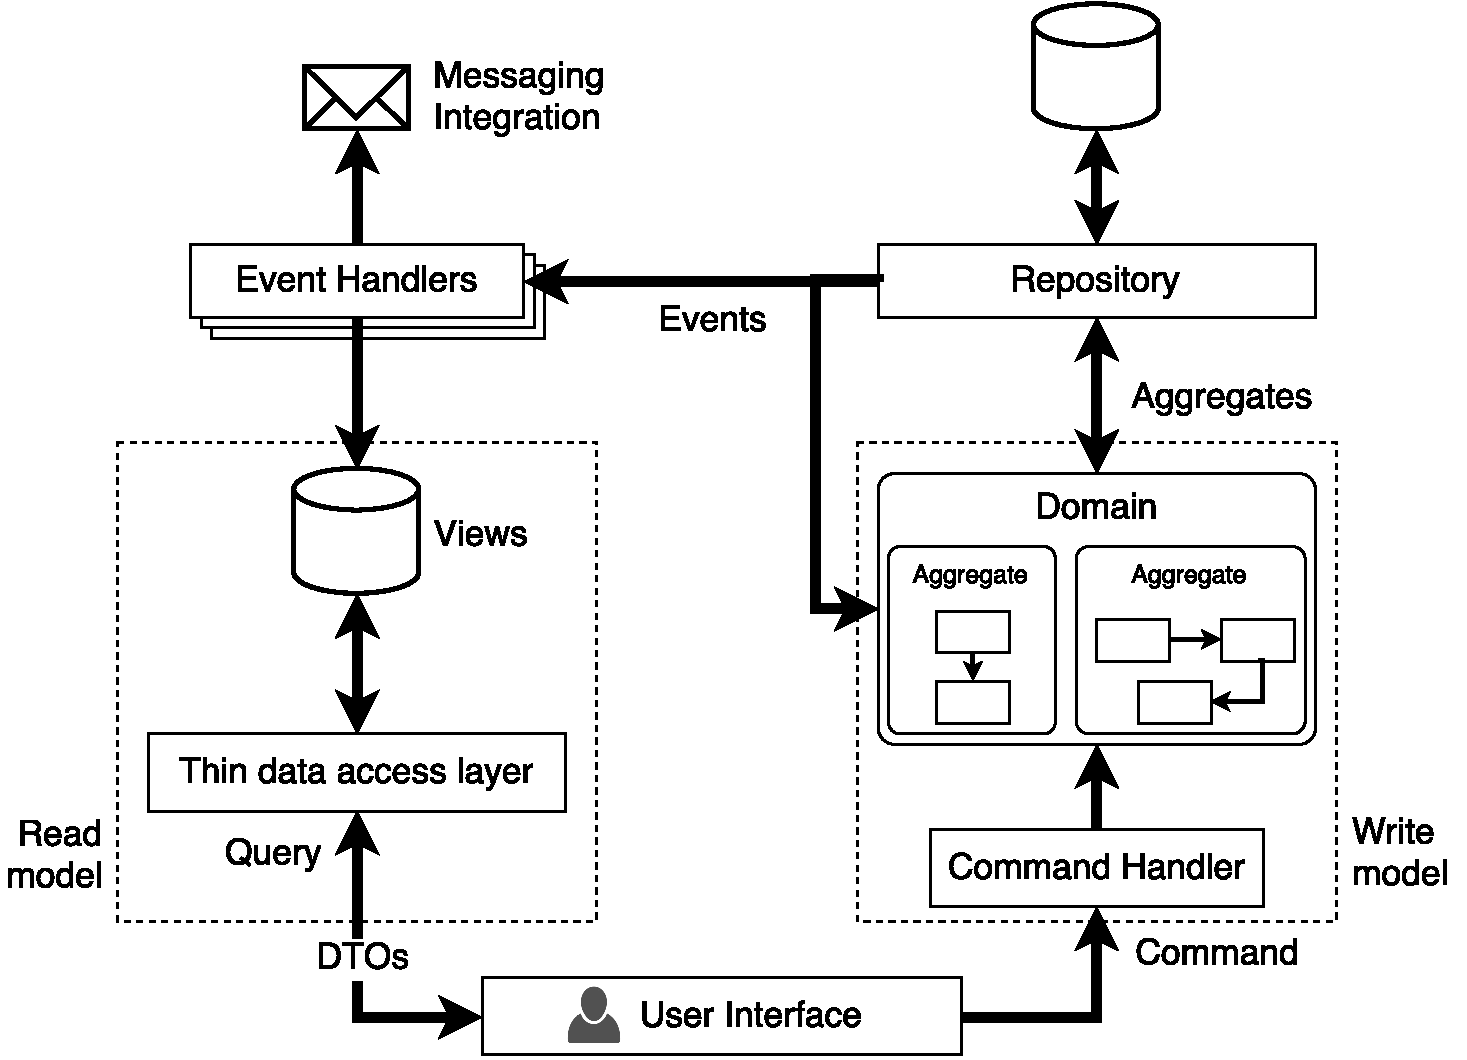
\includegraphics[width=0.84\columnwidth]{figures/cqrs-detail/cqrs-detail}
\caption{View of the CQRS design in detail%
}
\end{center}
\end{figure}

\subsection{CQRS with Event Sourcing}\label{cqrs-with-event-sourcing}

Let's revise what was said about CQRS (designed using DDD) and Event
Sourcing and describe how the two patterns connect together.

CQRS in its core is as simple concept as separation of read and write
models for purpose of scalability and performance in multi-user
collaborative environment. Domain-driven design fits nicely to this
paradigm with the domain model being the core of the CQRS write model.
Commands and events then manage state transition of the aggregates and
creation of read models respectively; also, they can be used to
communicate between aggregates and integrate other systems through
messaging protocols.

In a simple CQRS implementation without Event Sourcing the state of the
whole tree of aggregate's objects (entities, value objects) are
persisted to storage. If the state of the aggregate is to change, it is
loaded again, usually by a command handler, and an appropriate method is
called that changes the internal state of the aggregate. After that, the
aggregate is persisted again. Object-relational mapper (ORM) can be used
to save the objects to desired storage. The process is shown in Figure~\ref{fig:cqrs-no-es}.

In the case of event sourcing, the process flow is a bit different. The
events are used to recreate the state of aggregates instead of loading
the aggregate by ORM. These events are generated by the methods that
handle the state change of the aggregate triggered by the command
handlers. Instead of changing fields of aggregate entities or creating
new value objects directly, a new event representing the state
transition is created and applied to the aggregate. Applying the event
results in calling the appropriate event handler in the aggregate that
actually changes the state.

Now when the aggregate is loaded, instead of using ORM layer, all the
events published by the aggregate in the past are read and applied to a
completely new aggregate instance. By applying all the events one by
one, their event handlers are called appropriately and the aggregate
gets to the desired state to possibly process a method triggered by a
command. After the command was handled, we do not save the state of the
aggregate, but instead, all the new events marking new state changes
that were applied to that aggregate are persisted to the event store.
The event-sourced model is shown in Figure~\ref{fig:cqrs-es}.

From the perspective of command handling you can see that event sourcing
didn't bring any benefit; instead of mapping the whole object from ORM
repository, it just continually builds the aggregate from a stream of
events. And instead of saving the whole state of the aggregate, the new
events that the aggregate published are saved. The benefit lies in that
the structure of the aggregate is not bound to the ORM layer and can be
changed anytime, for example, to fulfill new requirements. Also, testing
of the domain model gets easier as the events can be used to set up the
test, so they represent various use cases and situations in the domain.
After processing a command under test, the published events are
asserted. Another thing is that the events are stored and can be used
for offline or batch processing, e.g.~reports or monitoring which do not
need to be updated in real-time.


\begin{figure}[h!]
\begin{center}
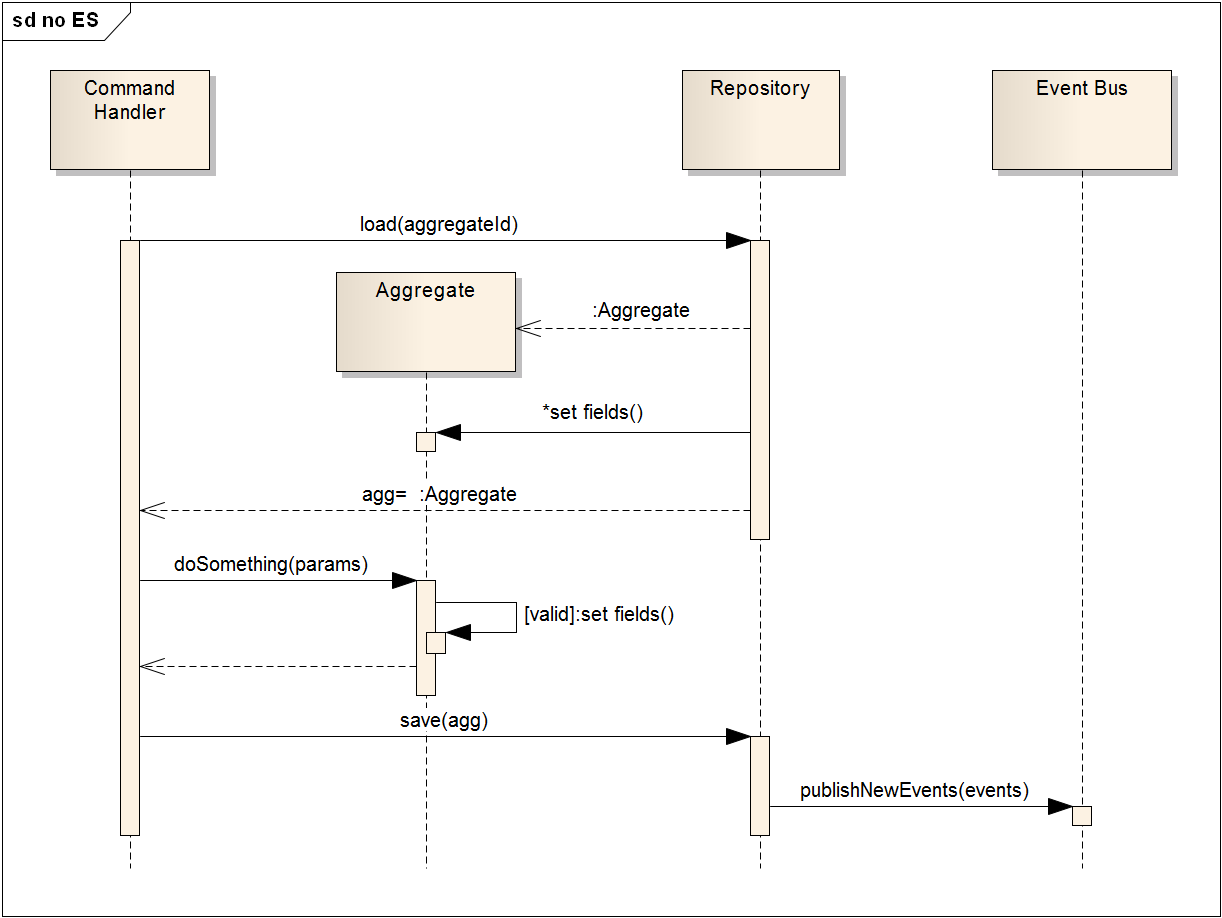
\includegraphics[width=0.98\columnwidth]{figures/cqrs-no-es/cqrs-no-es}
\caption{Handling aggregate state change in simple CQRS without Event Sourcing%
}
\end{center}
\end{figure}

\begin{figure}[h!]
\begin{center}
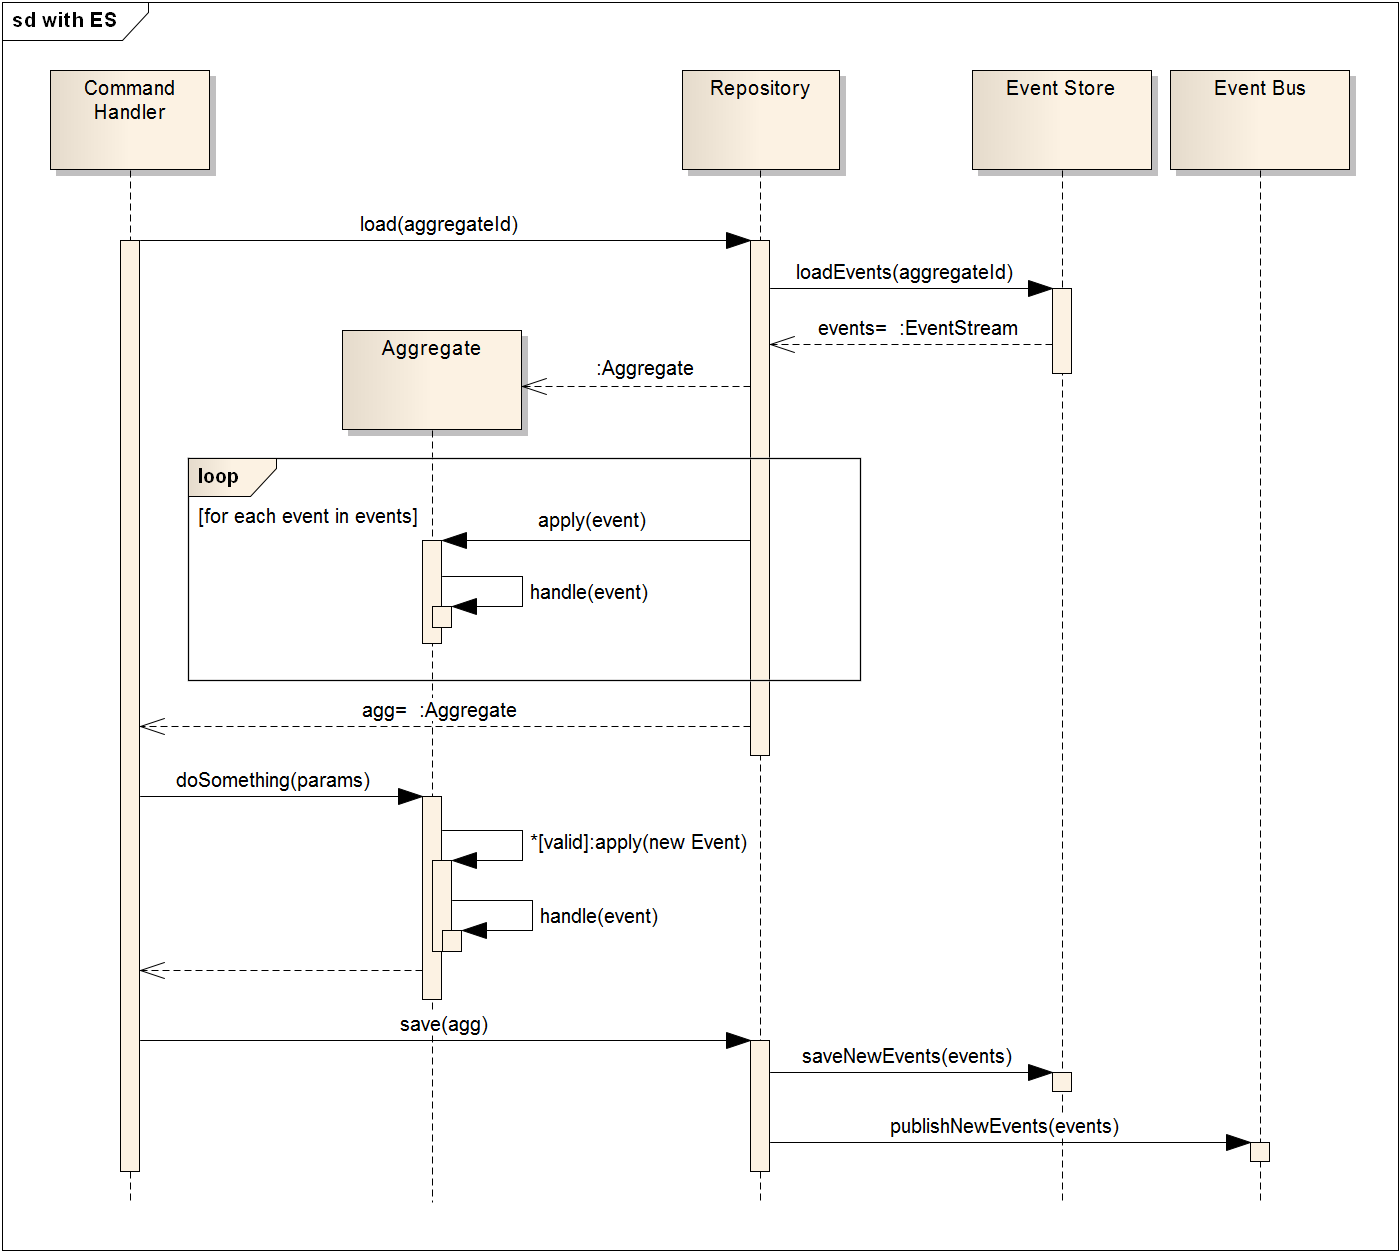
\includegraphics[width=0.98\columnwidth]{figures/cqrs-es/cqrs-es}
\caption{Handling aggregate state change in CQRS while using Event Sourcing%
}
\end{center}
\end{figure}

\subsubsection{Conflicting changes}\label{conflicting-changes}

CQRS with Event Sourcing, on top of the benefits presented above,
provides a great way of dealing with conflicting changes in one
aggregate. This usually happens when two users want to modify data on
the same aggregate nearly at the same time. One way to solve this
problem is by versioning the aggregates. Every time the aggregate is
saved, i.e.~new events are stored and published in reaction to a
command, the version of the aggregate is incremented. When both users
are working with the aggregate of the same version and both send a
command to alter the state of the aggregate, we can send the aggregate's
version together with the command. In the command handler, we can assert
that the aggregate we want to load to process the command is of that
version and if not reject the command because of conflicting
modification.

A better way than just rejecting the command altogether is to resolve if
the changes caused by a command are in fact conflicting. An example of a
conflicting change can be that both users update the same field but to a
different value, e.g.~year of the product release. On the other hand, if
the changes are non-conflicting, e.g.~one user updates year of the
product release and the other fixes a typo in the product title, then we
can handle both commands successfully despite operating on the same
aggregate version. This conflicting modification can be determined by
comparing two lists of events. One list contains events saved by the
aggregate since the last known version (the unexpected events for the
command) and the second list contains new events applied by the command
the user sent. If there is a pair of events from both lists that are in
conflict (e.g.~two ``\emph{product release year changed}'' events), an
exception can be raised notifying about the conflicting changes.


\subsection{Summary}\label{summary}

In this chapter, we introduced Event Sourcing with the Command Query
Responsibility Segregation design pattern, both of which are very
abstract and fundamentally easy principles. The implementation of the
two was expanded by practitioners of Domain-Driven Design methodology
and is highly based on its terminology. A few benefits and arguments why
use the described patterns were presented for the readers to reason
about some of the problems that the pattern can help us solve.


\section{Preparation for the
implementation}\label{preparation-for-the-implementation}

In this chapter, preparation for the implementation of CQRS and Event
Sourcing in the Java programming language and their application to a
real software is described. An existing project was used as a base for
refactoring into the CQRS and Event Sourcing principles. The reason why
it was decided to refactor an existing project was to try CQRS and ES on
a real, non-trivial domain, however, building a project from the ground
up would take a lot of time. The existing project was meant to provide
some use cases and implementation, on top of which the CQRS and ES
infrastructure could be based. Also, as this project uses the
traditional layered architecture, it helped with the realization of the
differences between the two approaches that will be discussed in the
next chapters.

Before diving into the refactoring, let's start this chapter with a
description of finding a suitable Java framework that would support the
refactoring to the CQRS and ES principles. The chapter then continues
with the introduction of the base project to the reader. This includes
the description of the project's goals, its design and implementation
details \emph{before} the refactoring.


\subsection{Supporting Framework}\label{supporting-framework}

First, it was decided to look for frameworks that support the CQRS and
ES principles and minimize their complexity for the programmers on the
Java platform. The supporting framework should solve the common problems
like persistence, event sourcing, integration and messaging. The
framework should not make it difficult to integrate into an existing
project. In the case of this thesis, it should enable the refactoring of
Integration Portal.

There are few frameworks that enable CQRS and ES with various features
and in various states of quality. The following aspects were examined in
each of the frameworks to determine the fitness for the refactoring.

\paragraph{Compatibility with CQRS and
ES}\label{compatibility-with-cqrs-and-es}

The framework should support all the core details of CQRS and ES that
very described in the previous chapter. On top of that, it should take
into account implementation details such as support for database
transactions, messaging using JMS (or other messaging systems),
persistence, etc.

\paragraph{Integrability}\label{integrability}

The framework should be easy to incorporate into the existing code base
without being counterproductive in the process. This means it should not
dictate the use of specific implementations but rather be open to
various application designs and purposes.

\paragraph{Active development and
support}\label{active-development-and-support}

A very important aspect for programmers to build trust in any project is
its activity in development, whether it be an implementation of new
features or fixing of bugs. Also, user support and activity on forums or
issue trackers is expected for the long-running projects.

\paragraph{Documentation}\label{documentation}

Development with any given framework or library is usually very slow and
painful without (good) documentation. So the existence and the condition
of the documentation is another quality aspect for the desired
framework.

\paragraph{Popularity}\label{popularity}

The popularity of the framework should also be taken into account.
Although it does not serve any purpose in development with the
framework, it should be noted that popular frameworks might have better
chance to stay, be maintained, and get support from the developers or
other users.

\subsubsection{Axon Framework}\label{axon-framework}

Axon Framework \cite{axon} proclaims itself as a Java Framework for
scalable and high-performance applications and being focused on making
life easier for developers that want to create applications based on the
CQRS principles and concepts, i.e.~commands, events, aggregates,
entities, sagas, etc. On top of that, it also supports event sourcing.

It has released many versions in the past; the latest version at the
time of writing this thesis was 2.4.3. It is actively developed, a new
major version 3 is a work in progress. It has nice and detailed
documentation and a sample project to showcase the code. It aims to ease
the development of the domain model and business logic and shields the
programmers from the implementation traps of CQRS and ES.

The code of Axon Framework is carefully designed providing a few
extension points (e.g.~to JMS or Disruptor). It supports the Spring
Framework's configuration and dependency injection. It also uses Java
annotations for building the domain model and event listeners without
being tied to the Axon's specific logic. However, it does not try to
hide CQRS architecture details or its components, so it is better to
have the knowledge of CQRS.

The code repository on GitHub has more than 300 stars and 100 forks
\cite{axon-repo}. The user community is active on the mailing lists and
on the issue tracker. The code is open source under the Apache 2
license. The authors also provide commercial services such as support
contracts, training, and consultancy.

\subsubsection{EventStore2}\label{eventstore2}

EventStore2 \cite{eventstore2} is a framework for creating event sourced
applications in Java. Much like Axon Framework it uses CQRS concepts and
terms for the implementation, and it utilizes the Java annotations to
configure command handlers, sagas and event handlers (called Projections
here). For asynchronous execution and clustering support it uses Akka, a
toolkit and runtime for building highly concurrent, distributed, and
resilient message-driven applications on the Java Virtual Machine (JVM).

It is in active development, with the current stable version being
2.4.3. A big disadvantage is a lack of detailed documentation. The whole
framework is described just in few paragraphs in a README file with few
examples of how to implement command handlers and projections. The
documentation totally omits how to use sagas, transactional support,
persistence, configuration and more.

The code base is hosted in a GitHub repository. It has 24 stars and 2
forks. The issue tracker does not contain any issues, not even closed.
No official website or any other references where found on the Internet.
From this, it was deduced that the framework is not actively used by
many users. It is open source under the MIT license.

\subsubsection{Jdon Framework}\label{jdon-framework}

The Jdon Framework \cite{jdon} website describes the framework as a Java
reactive framework that can be used to build Domain Driven Design
applications using CQRS and Event Sourcing with asynchronous concurrency
and higher throughput. It uses reactive approach and actor based model,
similarly to EventStore2 which uses Akka. It supports dependency
injection and annotation support and is integrable with Spring
framework.

The documentation is comprehensive and uses images to better explain the
principles. Typographically, however, it is in a poor state for reading
--- often the text is broken, it contains typos and grammar errors. On
top of that, the framework does not seem to be developed anymore. The
last change made to its code was two years ago. The latest stable
version 6.8 was released around that time too.

The framework's code is stored in a GitHub repository with 278 stars and
148 forks. A few issues are in the issue tracker, some written in
Chinese. The latest issues are asking about the activity of development,
but without any responses. It is open source under Apache 2 license.

\subsubsection{Summary and framework
selection}\label{summary-and-framework-selection}

Since CQRS and event sourced applications are not very common in the
Java world, not many frameworks exist. In the search for these
frameworks on the Internet, I focused on projects that aim to be used by
many users (not sample or ``playground'' projects of one author) with
good documentation and active development. The three frameworks I found
that were worth to study are described above.

EventStore2 and Jdon both use actor model and reactive approach
\cite{actor} for concurrent execution, where Akka seems to dominate the
Java (and Scala) world in that matter nowadays. Even though I would very
much like to get into reactive programming in Akka, the two frameworks
were found unconvincing to be chosen for the refactoring.

EventStore2 is actively developed but does not provide any other support
(as in the documentation, forums, mailing lists or website) and it also
lacks user base. On the contrary, Jdon Framework didn't lack these
things but it seems to have completely stopped the development without
any message to the users, and there are even no responses to new issues.

Axon Framework, on the other hand, excels in almost all the quality
aspects that were inspected. The downside is that it doesn't use actor
model or reactive programming. It is more conservative which can be
advantageous in some cases. Thus, Axon Framework was chosen to support
the refactoring of Integration Portal to CQRS and Event Sourcing.


\subsection{Axon Framework}\label{axon-framework}

In this section, let's introduce the reader to Axon Framework's
specifics that relate to the refactoring to CQRS and ES further in the
text. For more details, see the framework's documentation \cite{axon}.

As mentioned previously, Axon Framework very well supports Spring
Framework, which is also used in Integration Portal. It is not required
to use Spring Framework in order to use Axon Framework, however, it
greatly simplifies the configuration. Axon provides namespace support
for Spring XML configuration of the Application Context to set up the
Axon's building blocks.

Axon Framework doesn't hide the CQRS details from its users and so it
shares the CQRS terminology. The building blocks described in
\ref{command-query-responsibility-segregation}
\nameref{command-query-responsibility-segregation} are used to build the
domain model with Axon Framework. On top of these building blocks, some
infrastructure and configuration is needed to set up Axon. The following
paragraphs describe the concepts that are specific to Axon Framework
implementation.


\subsubsection{Command handling}\label{command-handling}

As previously described, a state change in CQRS starts with a command.
To represent a command, that can be handled by Axon, any Java object can
be used. Various types of commands can be represented by different
classes, e.g. \texttt{AddProductToCartCommand} or
\texttt{UpdateProductPriceCommand}. The class name captures the intent
of the command and the fields in the class instance carry the command
data. For example, the \texttt{UpdateProductPriceCommand} class could
have fields for the new price of the product and for the unique
identification number (ID) of the product that the command targets. In
Java, the code of that class could look like in Listing~\ref{lst:priceCommand}.

\begin{lstlisting}[caption={An example of a command class in Axon},label={lst:priceCommand},captionpos=b,float,floatplacement=H]
class UpdateProductPriceCommand {
    
    private ProductId productId;

    private Money newPrice;

    public UpdateProductPriceCommand(ProductId productId, Money newPrice) {
        this.productId = productId;
        this.newPrice = newPrice;
    }

    // ... getters and setters ...

}
\end{lstlisting}

The command name, represented by the class name, captures the intent of
the command. It uses the imperative naming convention, in comparison to
the naming convention of events, which use the past tense instead.

The next paragraphs provide an overview of the components related to
setting up the infrastructure for command handling in Axon.

\paragraph{Command gateway}\label{command-gateway}

To dispatch the commands represented by class instances, Axon provides a
convenient interface called a Command Gateway. This interface defines
two methods to send a command, which is passed as an argument. The
\texttt{sendAndWait()} method is blocking, which means it stops the
execution of the caller until the passed-in command is resolved, and it
returns the result of the command execution. The other method,
\texttt{send()}, is the asynchronous counterpart, i.e.~non-blocking.
Axon provides a default implementation of this interface called
\texttt{DefaultCommandGateway}, or the users can provide their own
implementation to suit their needs. The commands passed to the Command
Gateway are then send to the Command Bus.

\paragraph{Command bus}\label{command-bus}

An entry point to the Axon's command dispatching mechanism is the
Command Bus. Its responsibility is to route the received commands to the
command handlers. Each command is always sent to the exactly one command
handler. The interface defines two methods for dispatching the commands,
which are designed with asynchronicity in mind. It also provides methods
for (un)subscribing the command handlers.

The \texttt{SimpleCommandBus} is the simplest implementation of the
\texttt{CommandBus} interface. It provides a way of intercepting the
command object before it is actually dispatched to the command handler.
To intercept the command, in order to modify, validate, or block the
command, the command bus needs to be configured with a
\texttt{CommandDispatchInterceptor}. Additionally, a Unit of Work, which
will be described further, is maintained for each sent command by the
bus.

There are other implementations of the \texttt{CommandBus} interface
provided by Axon. One of them uses Disruptor \cite{disruptor} which
takes a different approach to multithreaded processing to increase
performance. Another implementation provides distribution of command
buses and command handlers across different JVMs.

\paragraph{Command Handlers}\label{command-handlers}

In Axon, a Command Handler is an object that receives a command of a
specific type and takes action based on its contents. There are a few
ways to create a command handler. One is based on implementing the
\texttt{CommandHandler} interface and its \texttt{handle()} method to
process the given command. The command handler is then subscribed to the
command bus by specifying the type of the command it handles.

Sometimes it is beneficial to have multiple closely related command
handlers in one object. This approach can be achieved by using the
\texttt{@CommandHandler} annotation on methods to mark them as command
handlers. The type of the command that the method can handle is
determined by the type of the first parameter. The object can be a
simple POJO (plain old Java object) and only the method annotations
determine that they are command handlers.

The support for Spring framework enables automatic subscription of the
command handlers to the command bus when the object is turned into a
Spring bean. We can use the Spring's inversion of control container to
inject dependencies to the command handlers.

The dependencies for the command handlers are usually the aggregate
repositories, which handle loading of aggregates and persisting their
changes. As stated in the introduction to CQRS, command handlers are
supposed to load an aggregate instance, call a method on it, and save
the aggregate changes.

\paragraph{Unit of Work}\label{unit-of-work}

The processing of a command can be seen a single unit. Each time a
command handler executes, it is tracked in a Unit of Work. When command
handling is finished, the current Unit of Work is committed and all
actions are finalized. This means that aggregate repositories are
notified about the changes in aggregates to save them. In the case of
event sourced aggregates, the new events applied to the aggregates are
stored to the event store and published to the Event Bus.

Note that the Unit of Work is not a replacement for transactions.
However, the Unit of Work can be bound with a transaction by configuring
the transaction manager. This transaction will be started at the
beginning of the command handler execution and committed when finished.
If any exception is thrown during command handling, the bound
transaction is rolled back.


\subsubsection{Domain modeling}\label{domain-modeling}

In the introduction to CQRS, the building blocks used in the domain
modeling process were described. Two of the building blocks --- events
and aggregates --- play a major role in Axon Framework.

\paragraph{Events}\label{events}

As previously described, an event is a representation of a fact that
something has changed in the system. A typical source of events is an
aggregate. With every change in the aggregate, an event is raised. In
Axon framework, we can use any Java object to represent an event, so we
are not bound by any interface or abstract classes. We usually design
events as immutable Java classes. The class names should capture the
intent of an event, usually in the past tense by convention. It is
highly encouraged to make the class serializable. A concrete event,
represented by a class instance, contains the data describing the event.
An example of an event class is presented in Listing~\ref{lst:updatedEvent}.

\begin{lstlisting}[caption={An example of an event class in Axon},label={lst:updatedEvent},captionpos=b,float,floatplacement=H]
class ProductPriceUpdatedEvent {
    
    private final ProductId productId;

    private final Money newPrice;

    private final Money oldPrice;

    public ProductPriceUpdatedEvent(ProductId productId, Money newPrice, Money oldPrice) {
        this.productId = productId;
        this.newPrice = newPrice;
        this.oldPrice = oldPrice;
    }

    // ... getters ...

}
\end{lstlisting}

The event class in the example is very similar to a command class
presented previously. Although not enforced, it is good practice to make
domain events immutable. So the class fields are final, and let's assume
that the classes of the field types are immutable too.

In many cases, the data in a command and in the corresponding event,
which is created while executing the command, are identical, including
the fields. In the presented example, however, the event contains one
additional field that carries the price for the product before the
change. Of course, this field is not required by any CQRS principles,
but in some event handlers, it can be convenient to know the original
value.

\paragraph{Aggregates}\label{aggregates}

An entity or a group of entities, which is always kept in a consistent
state, is called an aggregate. The aggregate root is the object on top
of the aggregate tree that is responsible for maintaining this
consistent state. Classes and primitive types can be used to design an
aggregate's structure (entities and value objects).

In Axon Framework, all aggregate roots must implement the
\texttt{AggregateRoot} interface. This interface describes the basic
operations needed by the aggregate repositories to store and publish the
generated events. Aggregates are identified by an aggregate identifier.
This can be any object, but the following rules must apply:

\begin{itemize}
\tightlist
\item
  It implements the \texttt{equals()} and \texttt{hashCode()} methods to
  ensure equality comparison with other instances.
\item
  It implements a consistent \texttt{toString()} method.
\item
  It is serializable.
\end{itemize}

Axon provides a number of implementations of the \texttt{AggregateRoot}
interface, which can be extended by the programmer to create the desired
aggregate. One of the implementation classes is the
\texttt{AbstractAnnotatedAggregateRoot} class which uses annotations to
simplify the aggregate code and increase clarity. An example of an
aggregate root that extends this abstract class is in Listing~\ref{lst:aggregateRoot}.

\begin{lstlisting}[caption={An example of an annotated-based aggregate root class in Axon},label={lst:aggregateRoot},captionpos=b,float,floatplacement=H]
class Product extends AbstractAnnotatedAggregateRoot {

    @AggregateIdentifier
    private ProductId id;

    private String name;

    private Money price;

    public AbstractAnnotatedAggregateRoot(ProductId id, String name, Money price) {
        apply(new ProductCreatedEvent(id, name, price));
    }

    public void updatePrice(Money newPrice) {
        if (!price.equals(newPrice)) {
            apply(new ProductPriceUpdatedEvent(id, newPrice, price));
        }
    }

    @EventSourcingHandler
    public void handle(ProductCreatedEvent event) {
        this.id = event.getId();
        this.name = event.getName();
        this.price = event.getPrice();
    }

    @EventSourcingHandler
    public void handle(ProductPriceUpdatedEvent event) {
        this.price = event.getNewPrice();
    }

}
\end{lstlisting}

This simple example shows the \texttt{Product} entity class which serves
as the aggregate root. The class defines a few fields that represent the
current state of the aggregate. In this case, all these fields contain
value objects only. The first field, the \texttt{id} of the type
\texttt{ProductId}, is annotated with the \texttt{@AggregateIdentifier}
annotation, which means that this field acts as the aggregate identifier
for the repository in Axon. The \texttt{ProductId} type should follow
all the rules listed above in order for Axon to work properly.

Following the fields, there is the class constructor and the method
\texttt{updatePrice()}. Both of which represent the public interface to
access and change the aggregate state. In most cases these are called
from a command handler. The constructor creates a new aggregate
instance, and the method updates the product price of an instance.
Notice that their code does not change the state directly but it applies
new events instead. This follows CQRS and ES principles as events
represent the state transition.

Whenever a new event is applied to an aggregate, an event handler for
that event type is called in the aggregate. There are two event handlers
in the example that handle the respective events applied by the methods
above. An event handler is the place that actually changes the state of
the aggregate, i.e.~updates the fields or state of other entities in the
aggregate.

To make it clear, why event handlers handle the actual state change
instead of the methods that emit events, take Event Sourcing into
consideration. When the aggregate is being loaded by the repository,
instead of retrieving the current state of the aggregate, the event
sourcing repository gets only a stream of historic events instead. These
events are then applied to a brand new aggregate instance one by one,
causing the event handlers to execute. So, the event handlers are
responsible for getting the aggregate to the desired final state. This
means that the public methods are never executed when replaying the past
events from the repository. This is desired by design because otherwise
it would mean that new events could be emitted while processing historic
events, which would result in changing the history of the aggregate.


\subsubsection{Repositories and Event
Stores}\label{repositories-and-event-stores}

Repositories are responsible for providing access to aggregates. In
CQRS, they are part of the write model, because aggregates are used to
handle state changes. For any other queries, a read model should be
used. Typically, repositories are optimized for lookup of an aggregate
by its unique identifier only. Some repositories will store the state of
the aggregate itself (using ORM, for example) while others store the
state changes represented as events in an Event Store. The repository is
responsible for persisting the changes made to aggregates in its backing
storage.

\paragraph{Repositories}\label{repositories}

In Axon, repositories must implement the \texttt{Repository} interface.
This interface defines the \texttt{add()} method for persisting a new
aggregate instance, and two \texttt{load()} methods for retrieval of a
previously saved instance. The \texttt{load()} methods use an aggregate
identifier to load the desired aggregate instance. One of the methods,
however, has an extra \texttt{version} parameter, that can be used to
load an aggregate instance of a specific version. For more information
about the aggregate versioning, see \ref{conflicting-changes}
\nameref{conflicting-changes}.

For the purpose of event sourcing, Axon provides the
\texttt{EventSourcingRepository} which loads an aggregate instance by
replaying its historic events to get it to the desired state. Also, when
new events are applied to an aggregate instance, as a result of state
change during command handling, this repository is responsible for
persisting the new events when committed. This all is done seamlessly
without programmer's intervention.

\paragraph{Event Stores}\label{event-stores}

The \texttt{EventSourcingRepository} must be configured with a storage
mechanism that handles the actual loading and storing of the aggregate's
events. This mechanism is called an Event Store and there are several
implementations that can be used. The implementations differ mainly in
the backing storage that is responsible for persisting the events,
e.g.~file system, Mongo database, JPA, JDBC, etc.


\subsubsection{Event processing}\label{event-processing}

When an aggregate instance is successfully saved, whether by storing new
domain events or by storing the whole aggregate state, the generated
events need to be dispatched to other components, e.g.~query database,
search engines, external systems, etc. These components are called event
listeners and the dispatching is done by the Event Bus.

\paragraph{Event Bus}\label{event-bus}

The mechanism that dispatches events to the subscribed event listeners
is called the Event Bus. Axon provides two implementations,
\texttt{SimpleEventBus} and \texttt{ClusteringEventBus}. Both
implementations manage the subscription of event listeners and forward
all incoming events to respective listeners.

The \texttt{SimpleEventBus} is suitable for dispatching events
synchronously and locally on one JVM. It sequentially passes incoming
events to all the registered event listeners. The
\texttt{ClusteredEventBus} allows grouping of event listeners to
so-called clusters based on their properties and non-functional
requirements. It also supports dispatching events to different JVMs on
different machines.

\paragraph{Event Listeners}\label{event-listeners}

Event listeners are components that react to the incoming events. All
event listeners must implement the \texttt{EventListener} interface,
which describes a single method that receives the event as a parameter,
the \texttt{handle()} method. Implementing classes need to register with
an event bus, so they can receive the events published to the bus.

The \texttt{handle()} method sequentially receives all the events
published to the event bus. However, the implementing classes very
rarely need to listen to all the types of events. In order to pick just
the events the listener wants to process, the method becomes cluttered
with many if-else or switch statements. Fortunately, Axon provides
annotation based event listeners where multiple methods can handle
different events based on the type of the event (effectively, based on
the event class). The handler methods need to be annotated with the
\texttt{@EventHandler} annotation. In that case, the listeners can be
any objects not requiring to implement the interface. See Listing~\ref{lst:eventListener} for an example.

\begin{lstlisting}[caption={An example of an annotation-based event listener in Axon},label={lst:eventListener},captionpos=b,float,floatplacement=H]
class ProductEventListener {

    @EventHandler
    public void handle(ProductCreatedEvent event) {
        // code to handle the event
    }

    @EventHandler
    public void handle(ProductPriceUpdatedEvent event) {
        // code to handle the event
    }

}
\end{lstlisting}

On top of that, the Axon's Spring support makes it easy to integrate the
listeners with the Spring's IoC container. This support takes care of
registering the event handlers with the event bus, even though they do
not extend the \texttt{EventListener} interface. It also enables
injecting bean dependencies into the listener, so they can be used by
the handler methods.


\subsubsection{Managing complex business
transactions}\label{managing-complex-business-transactions}

In many cases, an atomic and consistent transaction isn't possible to
carry out, for example in integration with external systems. This is the
case where a coordinator that mediates this kind of business transaction
is needed and that can take compensating actions to resolve the failure
in a transaction if necessary. In CQRS, it is called a saga or process
manager. Axon provides an infrastructure to support sagas.

\paragraph{Saga}\label{saga}

A saga is a special type of an event listener that manages a business
transaction. Each transaction is handled by one instance of a saga. It
maintains a state needed to manage the transaction. Typically, a saga
has a start and an end, both triggered by events. All sagas must
implement the \texttt{Saga} interface.

Axon provides an implementation of the interface, called
\texttt{AbstractAnnotatedSaga}, that uses annotations to extend the
behavior of the saga instance. Similarly to annotated event handlers,
there is the \texttt{@SagaEventHandler} annotation that marks the event
handler method in a saga. There is also \texttt{@SagaStart} annotation
that signifies that the handler method is the starting point of new saga
instance.

On the other hand, the \texttt{@SagaEnd} annotation on an event handler
method causes the saga instance to end. Alternatively, there is the
\texttt{end()} method, that can be used to programmatically end the
saga, for example when some condition is fulfilled.

To save resources when publishing events to sagas, they can be
associated with certain properties. Only those events having the
properties of given value, which a saga instance is associated with, are
published to that saga instance. This way, the existing sagas won't be
flooded with all the published events, but just those that matter to
each saga instance. The association properties are specified by the
\texttt{@SagaEventHandler} annotation.

\paragraph{Event Scheduler}\label{event-scheduler}

Axon also supports scheduled events suitable for managing deadlines.
Imagine a long-running transaction that involves paying an invoice. The
deadline for paying an invoice can be several weeks. So, a saga can
schedule an event for publication in the future. When the time comes the
event is published and that triggers the associated event handler which
handles hitting the deadline.

The \texttt{EventScheduler} can be used to schedule events for
publication. A simple in-memory implementation by the
\texttt{SimpleEventScheduler} is suitable for non-critical short
deadlines. When JVM is shutdown, the scheduled event is lost. For more
distant deadlines, the \texttt{QuartzEventScheduler} can be used. It
uses Quartz as the underlying scheduling mechanism, which provides
persistence, clustering, misfire management and so on.

\paragraph{Saga Manager}\label{saga-manager}

The purpose of a saga manager is to route events to the appropriate saga
instances and to manage their life cycle. All saga managers must
implement the \texttt{SagaManager} interface. The
\texttt{AnnotatedSagaManager} is an implementation that uses annotations
on the annotated sagas to manage their life cycle and event routing. A
list of saga types is needed to configure the manager, so it knows what
sagas it administers. Also, a saga repository must be provided to the
manager.

\paragraph{Saga Repository}\label{saga-repository}

The responsibility of a saga repository is to store and retrieve saga
instances. As some sagas can run for a very long period of time, it is
reasonable to store the saga instances to a persistent storage. When JVM
shutdowns (e.g.~on application restart or failure), the sagas are safely
persisted and ready to be loaded when needed. Axon provides a number of
implementations that handle the responsibility with different backing
storages --- JPA, JDBC, and Mongo. The default saga repository is a
simple in-memory implementation. When this repository is used, a saga is
lost if JVM is shut down before the end of the saga.


\subsubsection{Testing}\label{testing}

\textbf{TODO}


\subsection{Introduction to Integration
Portal}\label{introduction-to-integration-portal}

As stated in the introduction to this chapter, the CQRS and ES patterns
were examined on an existing project. This section introduces the
project that was chosen for refactoring into the CQRS and ES principles.

The project, known under the working title Integration Portal, aims to
integrate several systems of the Czech Technical University (CTU) for
the purpose of file sharing and archiving. It is a web application where
users (members of CTU and externs) can upload, share and organize files
in a way that resembles a regular computer file system. The file data is
stored in a data storage infrastructure provided by the CESNET
association.

Please note that the project is still a work in progress and some of the
functionality and requirements described below are in preparation or
active development at the time of writing this thesis. The refactoring
to CQRS and Event Sourcing described further in this chapter deals only
with the working functionality at that time.

The system is divided into two parts. The first part is the front-end
user interface presented to users in their web browser. The second part
is the back-end server that integrates the systems and provides a
communication interface for the frontend.

\subsubsection{Frontend}\label{frontend}

The front-end presentation layer of the project is a client-side
HTML5/JavaScript application \cite{frontend} written using AngularJS
framework \cite{angular}. It is a so-called single-page application,
that means the browser loads the web page only once and all the other
communication is done using asynchronous calls to the server in the
background. The page refreshes the content for the user by dynamic
modification of the page using JavaScript.

The front-end part presents the users with the files they uploaded or
they have access to through the sharing functionality. It provides means
of interaction with the files, i.e.~moving, renaming, deleting,
organizing to folders, etc. It also includes a user interface for
logging into the system with user's credentials and a section for
administrators.

However, all the actual processing and state transitioning is done on
the back-end part and the frontend is only used for displaying the
content and sending the commands to the backend. The communication is
done using a REST API (Application Programming Interface).

Because the frontend is not really a subject of refactoring to CQRS and
Event Sourcing, it won't be discussed in any more detail. For more
information, see \cite{ddd}.

\subsubsection{Backend}\label{backend}

The back-end server application \cite{backend} uses a traditional
three-layer architecture in Java Enterprise Edition implemented using
Spring Framework and its supporting libraries for web development,
security, database access, and REST services. A PostreSQL database is
used to persist the application data.

One of the objectives of the server-side application is to integrate the
systems to accomplish the goal of file system management for CTU members
and externs. The systems are described below.

\paragraph{FELid}\label{felid}

A global authentication and authorization system of CTU academics and
students supporting single sign-on functionality. This system will be
used to authenticate the users of Integration Portal.

\paragraph{KOSapi}\label{kosapi}

The system that enables applications to access various types of
information, e.g.~student's details or subject schedules, through a
RESTful web service. This system will be used to retrieve a list of
organizational units of the faculty that map to faculty departments.
Each portal user belongs to one organizational unit. Organizational
units are assigned a quota on the amount of space that is available for
users' files.

\paragraph{CESNET}\label{cesnet}

An association of universities of the Czech Republic and the Czech
Academy of Sciences that operates and develops the national
e-infrastructure for science, research, and education. Integration
Portal uses CESNET's data storage to store file data. It provides a
communication interface to upload and download files and it also
supports two different types of media that the files can be stored to,
on-line and off-line. Their types differ in speed and capacity. Rarely
used files are automatically moved off-line to slow but high-capacity
magnetic tapes (a manual switch is also possible). In case the file is
needed again, it can be moved on-line seamlessly.

\subsubsection{Architecture}\label{architecture}

The architecture follows a typical setup for Java Enterprise Edition
applications called a three-tier architecture \cite{p-eap}, where the
client-side application written in AngularJS is the presentation tier,
the back-end server is the application tier and the PostreSQL database
server is the data tier. On top of that, Integration Portal communicates
with other external systems through various channels to accomplish the
integration goal. As this thesis focuses on refactoring of the back-end
server to CQRS and Event Sourcing, let's describe its implementation in
more detail.

The internal code of the back-end application is organized into logical
layers, an arrangement which is a widely adopted best practice in Java
EE application development under the name layered architecture (or
N-layer architecture). Each layer is responsible for some functionality
of the application without being mixed with the rest. The description of
the three layers found in the back-end application and their
responsibility is following.

\paragraph{The controller layer}\label{the-controller-layer}

The entry layer for the back-end application is formed by a number of
controllers which handle the requests to the server. In Integration
Portal, a REST API implemented using HTTP protocol is used to
communicate with the front-end application. So most of the controllers
are responsible for validating the HTTP requests, parsing the data sent
with them and passing the flow to the next layer. Also, the controllers
construct responses and send them back to the UI application.
Additionally, in case of any error in upper layers, the controllers are
responsible for sending correct status codes in the HTTP response. These
entry points to the back-end application are also protected by user
authorization mechanism, so not every user is allowed to call any
controller handler method. The controllers are implemented using Spring
Framework MVC support and the authentication and authorization by Spring
Security framework.

\paragraph{The service layer}\label{the-service-layer}

The service layer represents the interface through which the business
logic is invoked. It consists of services represented by classes that
implement operations in the business domain. The services are used by
the controllers to invoke the requested operation in the service layer.
The responsibility of this layer is to maintain the data consistency for
each operation and also controls the data modification for the data
access layer and integration with external systems.

\paragraph{The data access layer}\label{the-data-access-layer}

The last layer is responsible for the data access and storage. Most of
the data is stored in the PostgreSQL relational database. This layer
mainly consists of classes called Data Access Objects (DAO) that access
the data stored in the database through ORM framework called Hibernate.
The data is retrieved from the database using Hibernate and SQL, and
mapped to instances of appropriate Java classes called entities. The
entities are then used by the service layer to modify the data to
fulfill the business requirements. Finally, through Hibernate, this
layer saves the modifications again into the database.


\begin{figure}[h!]
\begin{center}
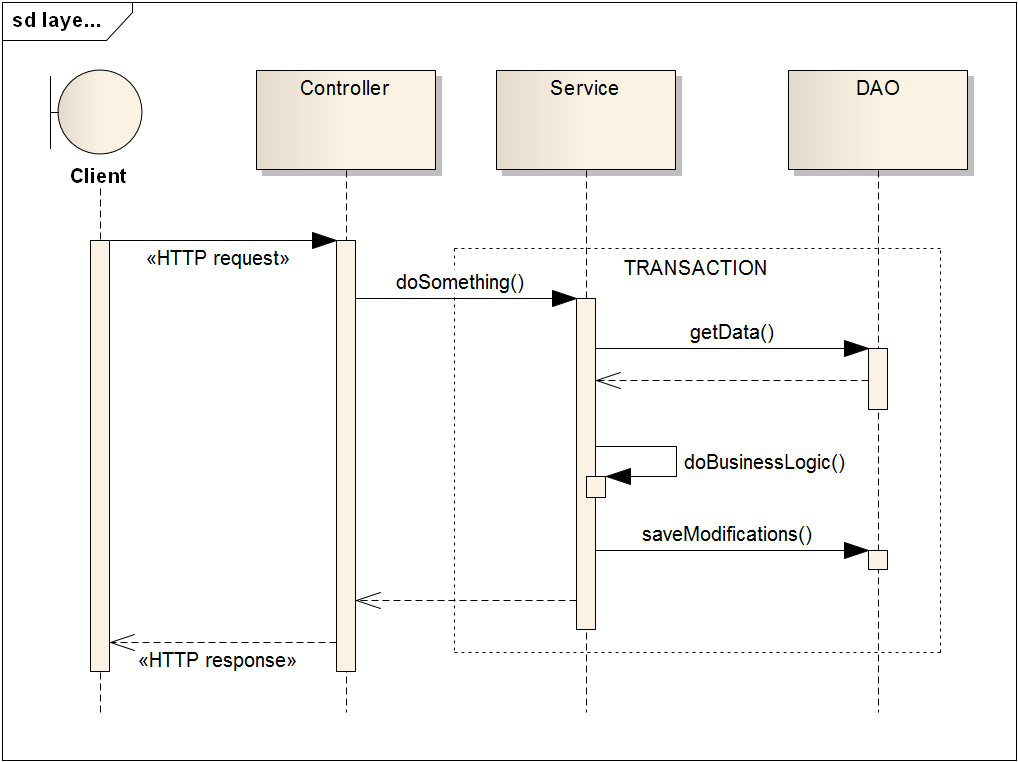
\includegraphics[width=0.7\columnwidth]{figures/layers/layers}
\caption{A typical communication flow between layers of the back-end server.%
}
\end{center}
\end{figure}

In Figure~\ref{fig:layers}, you can see a typical communication flow
between the described layers. The flow starts by an HTTP request to the
back-end server which is handled by the controller, then the operation
is delegated to a service class, which starts a database transaction.
The service executes the requested business operation which usually
involves retrieving data from the data access layer, modification the
data and finally saving the data back to the database. At last, the
database transaction is committed and an HTTP response is sent back to
the client.


\subsubsection{Domain model}\label{domain-model}

For the purpose of the refactoring to CQRS and Event Sourcing, it is
needed to describe the current domain model of the back-end application.
Please note that the domain model here depicts the model in a
traditional UML domain model diagram (shown in Figure~\ref{fig:domain}).
It is not meant to describe the domain model in terms of Domain-Driven
Development.

The domain model clearly captures all the entities and their
relationships within the business domain. The knowledge of the original
entities is important for the purpose of refactoring to CQRS where the
entities must be rethought in terms of aggregates.


\begin{figure}[h!]
\begin{center}
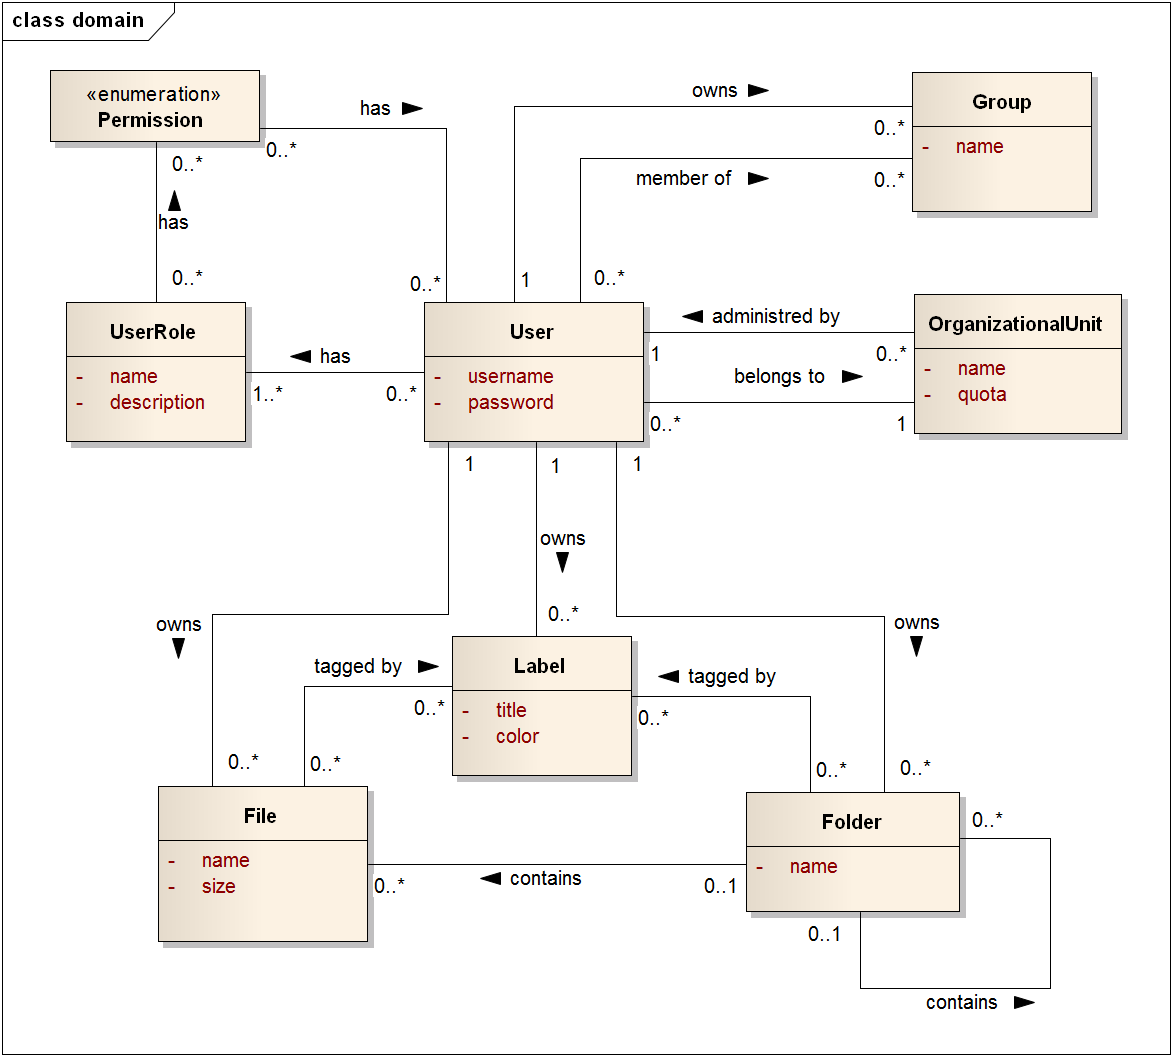
\includegraphics[width=0.98\columnwidth]{figures/domain/domain}
\caption{The domain model of the back-end application.%
}
\end{center}
\end{figure}

In the following paragraphs, a brief description of the entities of the
domain model is presented.

\paragraph{File}\label{file}

An entity that represents an uploaded file into the system. It's not
meant to carry the file contents, but it holds its metadata (file name,
size, content type, etc.). In the implementation, this entity is called
\texttt{FileMetadata} for historic reasons, but \texttt{File} captures
better that it represents a file in the simulated file system.

\paragraph{Folder}\label{folder}

The \texttt{Folder} entity is a way of organizing \texttt{File}s into
named groups and is equivalent to folders in regular file systems. A
folder can contain a number of files and also other folders effectively
creating a tree hierarchy of files and folders where files are the
leaves of the tree.

\paragraph{User}\label{user}

A \texttt{User} entity represents a user granted to access the system
and use it to upload and manage files and to organize them in folders.
The users become owners of the files they upload and folders they
create. At the time the refactoring to CQRS and ES started, there was no
sharing functionality, so the users can see only their files and folders
and no others in the frontend.

\paragraph{Label}\label{label}

Users can label files and folders with a user-defined text and color,
which are represented by the \texttt{Label} entity. This label is
displayed by the associated file or folder in the front-end part of the
system if the label belongs to the currently logged in user. Users can
utilize labels to visually orient themselves within the file system,
e.g.~by marking the files and folders that relate to ``work'' or
``school'' by an appropriate text and color. Also, users can search for
files and folders with a specific label.

\paragraph{Group}\label{group}

The \texttt{Group} entity is a way of organizing other users into named
groups. These groups are created and owned by users and are meant to be
a convenience for the sharing functionality in the future. If users want
to share a file or folder with a number of users, they can share it with
a group instead. This overcomes the complexity of selecting the users
for sharing one by one. The groups can represent individual research
teams or classes in the university.

\paragraph{Organizational Unit}\label{organizational-unit}

Organizational units map to the departments of the university. The
purpose of the \texttt{OrganizationUnit} entity is to group users of
Integration Portal to their appropriate organizational unit within the
university. Each unit is assigned a limit of file storage capacity their
users are allowed to utilize. This limit is called a quota. The sum of
sizes of all the files owned by the members of an organizational unit
must not exceed this quota.

\paragraph{User Role and Permission}\label{user-role-and-permission}

The \texttt{UserRole} entity and the \texttt{Permission} enumeration
form the authorization mechanism used to limit the user's access to
various features of the application (e.g.~administration). The
\texttt{UserRole} entity is represented by a name of the role and a
collection of permissions. The collection of permissions in a role
specifies what permissions a user has if associated with this role.
Additionally, a user can be assigned with extra permissions directly
without them being associated with any role. This way, it is possible to
combine direct permissions and role permissions to create a flexible
authorization system. Multiple roles and/or direct permissions can be
associated with a user.

\paragraph{Space}\label{space}

A space represents a category for files and folders and also specifies
the file repository used to store the file contents data. It is
represented as a simple string. At the time of implementation, it was
decided that Integration Portal could support multiple file repositories
than just CESNET in the future. It could be possible to integrate
multiple repositories to store the file data, e.g.~Dropbox, Google
Drive, One Drive, etc. Integration Portal would serve as a mediator to
transfer the file data between these repositories and, on top of it,
provide the sharing functionality and system integration. Space is not
represented as an entity in the domain model because it only specifies
the file repository for that file or folder. The frontend can display
different file trees based on the space the user selected. At the time
of writing this thesis, CESNET was the only file repository supported
and so there was only one space called \texttt{cesnet}.


\subsubsection{Functionality before
refactoring}\label{functionality-before-refactoring}

As stated previously, at the time of starting the refactoring to CQRS
and ES the project was still in development and some functionality was
not yet implemented. Some features were planned for implementation in
the future. The domain model described above illustrates the back-end
domain entities before refactoring. The implemented functionality around
these entities at that time is presented below.

\paragraph{User management}\label{user-management}

\begin{itemize}
\tightlist
\item
  User authentication with username and password (no FELid integration
  yet)
\item
  Authorization based on permissions to

  \begin{itemize}
  \tightlist
  \item
    access to the main administration (users, user roles)
  \item
    edit organizational units
  \item
    edit externs
  \item
    edit password
  \end{itemize}
\item
  Password change
\item
  Group management
\item
  User role management
\end{itemize}

\paragraph{Files}\label{files}

\begin{itemize}
\tightlist
\item
  Uploading (data being stored in CESNET infrastructure)
\item
  Renaming
\item
  Moving to other folders
\item
  Removing
\item
  Downloading the file contents
\item
  Updating the file contents
\item
  Switching to online / offline medium in CESNET
\end{itemize}

\paragraph{Folders}\label{folders}

\begin{itemize}
\tightlist
\item
  Creating
\item
  Renaming
\item
  Moving to other folders
\item
  Removing (along with all their child files and folders)
\item
  Switching to online / offline in CESNET
\end{itemize}

\paragraph{Labels}\label{labels}

\begin{itemize}
\tightlist
\item
  Creating
\item
  Modifying (text, color)
\item
  Deleting
\item
  Adding and removing labels on files and folders
\item
  Filtering files and folders by a label
\end{itemize}

\paragraph{Organizational Units}\label{organizational-units}

\begin{itemize}
\tightlist
\item
  Modifying (name, quota)
\item
  Assigning organizational unit administrators
\end{itemize}

\subsubsection{Missing functionality}\label{missing-functionality}

\begin{itemize}
\tightlist
\item
  Sharing files with other users
\item
  Enforcing the storage capacity limit of organizational units by their
  quota
\item
  KOSapi integration
\item
  FELid integration
\end{itemize}


\section{Refactoring of Integration
Portal}\label{refactoring-of-integration-portal}

Now that all the principles, concepts, and tools were settled and
explained, the whole process of refactoring the Integration Portal
application to the CQRS/ES design is presented. This section includes
describing the preparation and strategy chosen for the task, the sole
evolution of the refactoring, and propositions of solutions to some
problems that occurred in the process. In conclusion, a few ideas for
the future extensions of this design to implement new features is
suggested.

\subsection{Preparation}\label{preparation}

In the preparation to the refactoring, it was needed to go through the
whole back-end code to get knowledge of all the features and
functionality that would be subjected to the refactoring. In the
process, it was found out that some of the code needs to be revised to
better fit the CQRS design.

The first thing was to untangle the dependencies of the components and
layers to find out how they are connected and how it affects the
refactoring. In the original design, where CQRS and ES principles were
not taken into account, some of the code aspects were believed to cause
trouble in the refactoring. Because of that, the code underwent some
changes before the refactoring.

\subsubsection{Revising the REST
interface}\label{revising-the-rest-interface}

After reading \cite{journey}, the idea of a task-based user interface,
described in \ref{task-based-user-interface}
\nameref{task-based-user-interface}, was taken into consideration in
regards to the Integration Portal UI. A RESTful application programming
interface mediates the communication between the front-end user
interface and the back-end logic.

The API was designed according to the typical RESTful concepts. Every
entity in the backend (User, Folder, File, etc.) was represented as one
resource in the interface. The four basic HTTP methods --- GET, POST,
PUT, and DELETE --- were defined on most of the resources in order for
the UI to take actions on the entities in the backend. These methods
effectively convert to the known CRUD scheme (Create, Read, Update,
Delete). The create, read, and delete actions are usually
straightforward using the POST, GET, DELETE methods respectively.
However, a great care must be taken regarding the update action. There
are often multiple features on a resource that can be updated. With
CRUD-based REST interface, it is possible to use one HTTP method (PUT)
to modify multiple different components of one resource in a single
request (e.g.~change a folder name and set new label).

The design of general update command in RESTful API can be problematic
when using CQRS because the intent of the request becomes unclear. From
the perspective of the user interface, there is no real business logic
connection between changing a folder name and setting a new label at the
same time. Even the UI never sends one PUT request to alter multiple
unrelated features of one resource. So a general-purpose update request
on a resource is an exaggerated abstraction that hides the intent of the
change. The importance of capturing intents in commands and events is
explained in \ref{command-query-responsibility-segregation}
\nameref{command-query-responsibility-segregation}.

To solve this problem, it was decided to redesign the back-end REST API
so the update request carries the intent clearly with one component to
change at a time. A few ways how to carry out the redesign were
considered. They are described in detail further in ?REST
REDESIGN?\textbf{reference needed}. For now, let's just describe the
chosen way of the new arrangement of the REST interface.

First, all the modifiable features of each resource were collected. Each
feature was assigned a subresource of the original resource URL. To
carry the intent of the change, a POST request is sent on this newly
created URL for each feature. Consider the following example of REST API
interface to change a name of a folder resource:

\noindent Before the redesign

\begin{lstlisting}[caption={}]
PUT /folder/123
{"name": "New folder name"}
\end{lstlisting}

\noindent After the redesign

\begin{lstlisting}[caption={}]
POST /folder/123/nameChange
{"name": "New folder name"}
\end{lstlisting}

As you can see, the difference is made by a shift in the URL to target
one specific feature of the original resource. This way, changing
multiple features in one request is not possible. The
\texttt{nameChange} subresource expects modification of the name only
and thus carries the intent clearly --- it changes the name. The rest of
the modifiable features of each resource was redesigned in a similar
way.

\subsubsection{Revising the original domain
model}\label{revising-the-original-domain-model}

Concurrently with the refactoring, a development of a new feature was
planned to extend the functionality in the original code. The
functionality should have allowed users to share their files with other
users, which was not possible before. This also included the ability to
specify permissions on the shared files for each user (or group). The
responsibility of the development was assigned to another member of the
Integration Portal team. The time of completion of this functionality
was expected to be during the refactoring and thus, it was originally
intended to be part of the refactoring as well.

This resulted in some changes to the original domain model to support
this functionality. Specifically, there was a small issue in the design
of the entities in the original domain model that prevented sharing the
same code for both folders and files. This issue was even more
problematic for development of the new functionality.

Both folders and files represent nodes in the simulated file system
tree. Conceptually, they are very similar entities. They even share some
of their fields, like the name, parent folder, owner, assigned labels,
etc. However, they were originally designed as totally distinct entities
that did not share a common abstract class. This resulted in code
duplication in several places in the backend, as well as in the
front-end application. The same issue would be even more noticeable in
the planned file sharing functionality.

Thus, the two entities were rewritten to push the shared fields to an
abstract class called \texttt{Node} as shown in Figure~\ref{fig:node}.
This way a lot of redundancy was removed and the code became clearer. In
the end, the redesign was beneficial for the refactoring to CQRS too.


\begin{figure}[h!]
\begin{center}
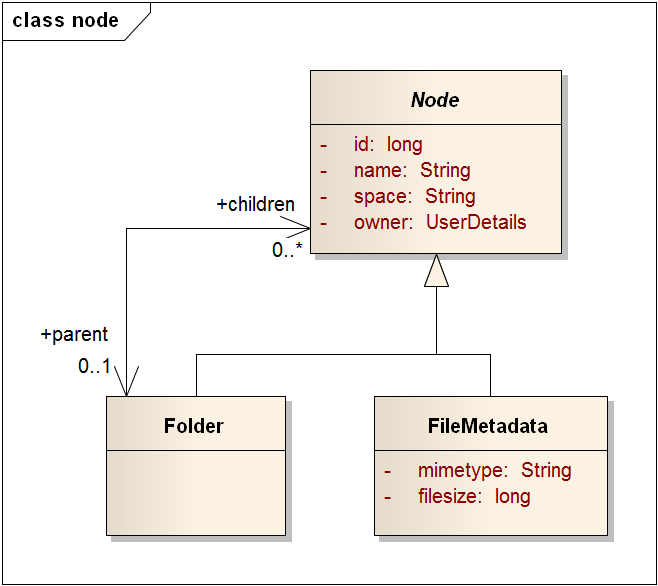
\includegraphics[width=0.49\columnwidth]{figures/node/node}
\caption{The domain model of the simulated file system after redesign%
}
\end{center}
\end{figure}

\subsubsection{Refactoring strategy}\label{refactoring-strategy}

When the preparation phase was completed, the actual task of refactoring
the domain model and architecture to CQRS and Event Sourcing was ready
to be started. But before diving into it, a strategy, that would help in
the implementation, was thought through carefully.

It was decided to carry out the implementation in small portions, one at
a time. Each portion contained functionality regarding one entity, that
was subjected to refactoring, throughout all the layers, i.e.~the
service, controller, and data access layers, and the data transfer
objects for REST API (called representations).

The strategy was to ensure compatibility with the original design so the
process of refactoring was easier and less extreme. This allowed the
system to stay in one coherent form without changing the backing
infrastructure and the deployment process. That means, that after the
refactoring, the backend was still one module without asynchronous
execution, messaging systems or read model processors running on
different machines.

For the read model built by CQRS, a PostgreSQL database, the very same
as in the original design, was used. The read model was built using the
Hibernate ORM in the same way as in the original design. So, the queries
for the CQRS and the original design remained more or less unchanged.
This allowed me to focus on the refactoring of the write side,
i.e.~creating the domain model, processing of commands, and emitting
events (used to build the read model).

Because the system had been rewritten gradually, i.e.~CQRS/ES was
applied to one domain entity at a time, and by using the same database
schema for the read model, the system worked even though it was only
partially refactored. The original features that were not refactored yet
used the database to process both commands and queries. The refactored
features, however, processed the commands by utilizing the new write
model build by using Axon Framework, and emitted events were used to
build the read model, which was compatible with the original design. So,
the database shared the data between both the original implementation
for the joint read-write model and the refactored implementation for the
CQRS read model only. For simplicity, the schema of the database was
altered for the database to act as an event store too.

Another important decision, in the strategy of refactoring to CQRS and
ES, was incorporating Test-Driven Development (TDD) \cite{tdd} into the
process. Tests were often written first to reason about the changes, and
then continually run in the process of refactoring to ensure the
implementation of some feature was correct. These tests were integration
tests and were based on the tests written for the original design. The
system was tested as a black box, where a command was an input and the
database state was the output. This way it was guaranteed that the read
model for CQRS and the joint read-write model for the original design
were in the correct state for both implementations to function properly.

Using this strategy, the result of the refactoring was a system based on
the CQRS and ES principles, but that used the original database and the
transactional, local-JVM, and synchronous execution for its read model
the same way as the original design. This strategy was easier for the
refactoring to reason about by making small steps and by using tests to
ensure the system works as before, which is fundamental in any
refactoring. The final state of the refactoring enables the system to
easily divide the backend to several modules (or create microservices),
integrate message queue systems, asynchronous execution to improve
scalability and flexibility. All this can be done just by modifying the
Axon Framework configuration and by making changes to the infrastructure
and deployment, but the code can remain almost the same.


\subsection{Refactoring the domain
model}\label{refactoring-the-domain-model}

As described in \ref{introduction-to-integration-portal}
\nameref{introduction-to-integration-portal}, the original domain model
consisted of Hibernate entities that were modified by the business logic
in the service layer and persisted by the data access layer. The
refactoring of functionality for each entity is described in the
following paragraphs.

The side effect of carrying out the strategy outlined above is that most
of the original queries to the system remained unchanged after the
refactoring. This means that the way the data are queried is more or
less the same as in the original design --- query the data access layer
for the data stored in the database, then map the data to the respective
DTOs so they can be converted to JSON and sent to the client.

The methods responsible for carrying out the business logic, however,
were rewritten from scratch to follow CQRS principles. In the following
text, the changes made to the code are described.

\subsubsection{Service layer}\label{service-layer}

In the original design, the service layer was an interface used for both
accessing the data and invoking the business logic. A few of the methods
used both responsibilities mixed together --- the business logic made
some modifications to the data and the result was sent to the client
(often the whole entity representation was returned as per RESTful
conventions).

This interface was being accessed by the controllers, which either only
returned the queried data or invoked the requested business logic and
returned the outcome. Accessing the service layer methods starts a
transaction. Transactions were needed by both responsibilities --- while
updating the database entities needs a transaction on its own, the
queries need a Hibernate session, which can be accessed by starting a
read-only transaction.

In the process of refactoring, the interface of this layer was preserved
and modified only slightly to reflect changes in the refactored domain
model. Changes to the implementation related mainly to the non-query
methods. Transactional behavior was removed from these methods because
managing the transactions in the business logic is now the
responsibility of Axon's command handlers and their unit of work. The
query methods as stated above remained almost unaffected by the
refactoring.

The implementation of the original non-query methods was altered so they
don't execute any business logic directly. Instead, the execution was
delegated to the command handlers and aggregates in the new domain
model. The responsibility of the methods now is to instantiate a new
command with correct data (usually passed as method arguments) and send
them through the command gateway to the respective command handler that
processes the command.

An important change from the original implementation is that the service
methods that are responsible for creating new domain objects
(aggregates) are now also responsible for creating their unique
identifier (ID). In the original design, this was done by the database
when persisting new entities just by incrementing the table's internal
sequence number. In the new implementation, IDs are randomly generated,
before the command is dispatched, using a statistically safe algorithm
and then used to reference the aggregate.

To summarize, the interface of the service layer remains almost
unaffected by the refactoring and is still used by controllers in the
same way as in the original design. The implementation of the business
logic methods, however, changed to delegation of the processing to the
new domain model by dispatching commands. An example of such method is
shown in Listing~\ref{lst:serviceMethod}.

\begin{lstlisting}[caption={An example of a business-logic service method after refactoring},label={lst:serviceMethod},captionpos=b,float,floatplacement=H]
public void deleteLabel(String labelId) {
    commandGateway.sendAndWait(new DeleteLabelCommand(
            LabelId.of(labelId)
    ));
}
\end{lstlisting}


\subsubsection{The domain model}\label{the-domain-model}

The entities of the original domain model remained to be used for
building and querying the read model. However, the business logic, which
was used to modify the entities, moved to the new domain model designed
according to DDD principles by using Axon Framework and driven by
commands.

The entities and their business logic in the original implementation
were examined and rewritten to aggregates and their behavior. As an
example, let's describe the transformation of one simple entity ---
\texttt{Label}. Refactoring of the rest of the entities would follow the
same scheme.

Labels can be assigned to (or removed from) folders and files (nodes)
and they are owned by one user. A user can change a label's color and
name, or delete it. Of course, by deleting, it the label is removed from
all the assigned folders and files. To reference one concrete label
(e.g.~in the REST API), a unique ID is set to the entity.

In the original design, the \texttt{Label} entity was modeled as a
Hibernate entity that exposed only getter and setter methods. The
business logic was placed in the service layer, specifically to the
implementation of \texttt{LabelService}.

This entity and the behavior can be easily transformed to an aggregate.
The way that aggregates are designed follows the traditional non-anemic
OOP principles, i.e.~objects with both state and behavior. The
\texttt{Label} aggregate would be modeled in UML like in Figure~\ref{fig:label}. The fields that represented the original entity are
specified in the aggregate as well and the business logic moved from the
service layer to the aggregate.


\begin{figure}[h!]
\begin{center}
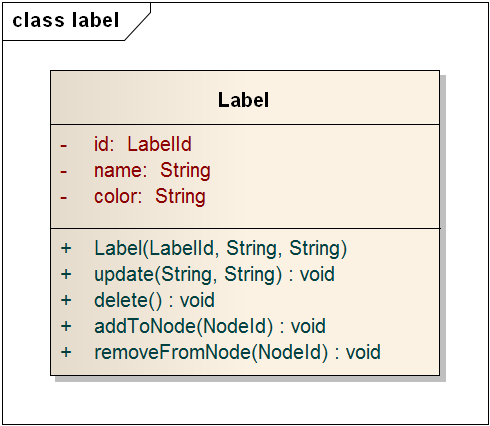
\includegraphics[width=0.35\columnwidth]{figures/label/label}
\caption{Label aggregate%
}
\end{center}
\end{figure}

As you can see, the interface is quite straightforward. There is a
constructor that receives all the information to create a label (ID,
name, and color). Following that, the signatures of methods that change
the aggregate's state are defined. Notice that these methods are not
setter methods like in Hibernate entities, but they represent various
operations in business logic of the aggregate. These operations more or
less copy the intents of respective commands, which will be described
further in the text.

The implementation of the aggregate is influenced by the CQRS and ES
principles, i.e.~an event is emitted for each state change. An event can
be processed by one event handler in the aggregate, which actually
changes the aggregate's state (updates the values of the aggregate's
fields). See the implementation in TODO PRILOHA X \textbf{reference needed}.
The class for the event that gets emitted in the \texttt{update()}
method is presented in Listing~\ref{lst:labelUpdatedEvent}.

\begin{lstlisting}[caption={The \texttt{LabelUpdatedEvent} class},label={lst:labelUpdatedEvent},captionpos=b,float,floatplacement=H]
@Value
public class LabelUpdatedEvent {

    private final LabelId id;

    private final String name;

    private final String color;

}
\end{lstlisting}

Note that the class is actually not compilable by the standard Java
compiler. There are some final fields but no constructor to initialize
them. But notice the \texttt{@Value} annotation. This annotation is part
of Lombok library \cite{lombok} that aims to reduce the number of
repeated tasks and constructs needed by a developer to write a proper
Java class. At compile time, the annotation defines which missing
language constructs need to be added so the class compiles.

The \texttt{@Value} annotation says that the class is an immutable value
class, meaning that it is only a container for data. At compile time, it
generates a constructor, which initializes all the class fields, and it
also adds a getter method for each field. This greatly helped in
development to define a lot of classes (for commands and events) without
the need to write constructors for each class and getter methods for
each field. Via other Lombok annotations, the library is also used in
other places (e.g.~aggregates) where some constructs are repeated as
well.

However, this comes with a cost that the developer's IDE (Integrated
Development Environment) needs support for Lombok annotations so the
validation and code completion works. Usually, this support is brought
by some plugin or extension to the IDE. The successful compilation is
achieved by a compiler annotation processor provided by the library if
it is present on the classpath.


\subsubsection{Command processing}\label{command-processing}

To send the commands that invoke business logic on an aggregate, the
service layer was modified as previously explained. Expanding on the
example of the label functionality, let's describe the transformation of
the \texttt{LabelService} implementation regarding a creation of a
label. Originally, the responsibility of the service implementation was
to retrieve the \texttt{Label} entity (or create a new instance), do
some business logic that modified the entity, and finally save the
result to the database. After refactoring, the business logic methods
turned into factories of commands that are sent to the Axon's command
gateway to be dispatched. Consider, for example, the
\texttt{createLabel()} method presented in Listing~\ref{lst:createLabelMethod}.
After refactoring, it only delegates the execution of business
logic using a new command instance that is sent to the command gateway.

\begin{lstlisting}[caption={The \texttt{createLabel()} service method after refactoring},label={lst:createLabelMethod},captionpos=b,float,floatplacement=H]
public void createLabel(String name, String color) {
    String id = UUID.randomUUID().toString();

    commandGateway.sendAndWait(new CreateLabelCommand(
            LabelId.of(id), name, color
    ));
}
\end{lstlisting}

As you can see, apart from sending a command, it also creates an
identifier for the new aggregate instance being created by the command.
This is a change from the original design, where ID was created by the
read/write database on insertion. As the read model is now a side effect
of processing events, the identifier needs to be created beforehand.
This also makes scaling and asynchronous command processing easier,
because the ID is known before any read model is updated, and it can be
returned to the client immediately.

\begin{lstlisting}[caption={The \texttt{CreateLabelCommand} class},label={lst:createLabelCommand},captionpos=b,float,floatplacement=H]
@Value
@EqualsAndHashCode(callSuper = true)
public class CreateLabelCommand extends UserAwareCommand {

    private final LabelId id;

    private final String name;

    private final String color;

}
\end{lstlisting}

The dispatched command, defined by the class in Listing~\ref{lst:createLabelCommand}, is forwarded to the command bus
(\texttt{SimpleCommandBus}) which executes the respective command
handler. But just before that, it is intercepted by
\texttt{AddUserCommandDispatchInterceptor}. As you can see, the command
class extends \texttt{UserAwareCommand}, which is an abstract class that
adds the \texttt{sentBy} field. This field is intended for holding the
identifier of the user that issued the command. To reduce code
duplication of setting the identifier of the currently logged-in user to
every command, the interceptor is used to set the user identifier just
before it is dispatched by the command bus. Also, notice that the
command class is also declared with the \texttt{@Value} and
\texttt{@EqualsAndHashCode} annotations from Lombok library.

Most of the time, command handlers follow the same pattern---load the
aggregate from the repository, call a method on the aggregate, and
finally, save the aggregate back to the repository. The actual storing
mechanism depends on the repository type (e.g.~event sourcing
repository). However, in case of the commands that create aggregate
instances, the command handler must instantiate the aggregate and add it
to the repository. The implementation of the command handler for
\texttt{CreateLabelCommand} is presented in Listing~\ref{lst:createLabelCommandHandler}.

\begin{lstlisting}[caption={The command handler for \texttt{CreateLabelCommand}},label={lst:createLabelCommandHandler},captionpos=b,float,floatplacement=H]
@CommandHandler
public void createLabel(CreateLabelCommand command) {
    checkUnique(command.getName(), command.getColor(), command.getSentBy());

    Label label = new Label(
            command.getId(),
            command.getName(),
            command.getColor(),
            command.getSentBy()
    );

    repository.add(label);
}
\end{lstlisting}

A command must be valid so it can be processed by a command handler. In
this case, the command handler checks that a label with the given
attributes does not exist yet (as label's name and color are unique per
user). Then it creates a new \texttt{Label} aggregate by calling the
constructor. The constructor applies the \texttt{LabelCreatedEvent} in
the process. Finally, the aggregate is added to the repository. As the
repository for Labels uses event sourcing, it saves the applied event to
the event store.


\subsubsection{Event processing}\label{event-processing}

When the command handler successfully finishes, that is after saving or
adding the aggregate to the repository, the new events generated by the
aggregate are sent to the event bus. To ensure the synchronous,
local-JVM, and transactional execution when creating the read model (as
per the strategy), the \texttt{SimpleEventBus} was used. A number of
event handlers are registered to the event bus using Axon's Spring
integration support. In all Spring beans, methods annotated with the
\texttt{@EventHandler} annotation receive the respective events as the
first attribute.

The majority of event handlers created in the refactoring have only one
purpose and that is to build the read model the same way as in the
original design. This was achieved by moving the original code, which
modified the Hibernate entities, from the service layer to the event
handlers. As the business logic and invariant rules were already taken
care of by the aggregates in the new domain model, the responsibility of
event handlers is just to update the Hibernate entities to reflect the
changes represented by the events. Let's finish the example of creating
a label with the handler for \texttt{LabelCreatedEvent} shown in Listing~\ref{lst:labelCreatedEvent}.

\begin{lstlisting}[caption={The event handler (listener) for \texttt{LabelCreatedEvent}},label={lst:labelCreatedEvent},captionpos=b,float,floatplacement=H]
@EventHandler
public void createLabel(LabelCreatedEvent event) {
    UserDetails owner = userDao.getReference(event.getOwner().getId());

    Label label = new Label();
    label.setId(event.getId().getId());
    label.setOwner(owner);
    label.setName(event.getName());
    label.setColor(event.getColor());

    labelDao.save(label);
}
\end{lstlisting}

The event handler uses the original Data Access Objects from the data
access layer to communicate with the Hibernate ORM. To correctly set up
the label's relationship with the owning user, a reference of the
\texttt{UserDetails} entity is created from the user identifier. The
entity is then initialized with the data from the event and with the
\texttt{UserDetails} entity reference and finally persisted.

A similar pattern is found in all the other event handlers that build
the read model.


\subsubsection{Overview of the refactored
code}\label{overview-of-the-refactored-code}

An overview of the package structure and dependencies regarding labels
after refactoring is shown in Figure~\ref{fig:package}.


\begin{figure}[h!]
\begin{center}
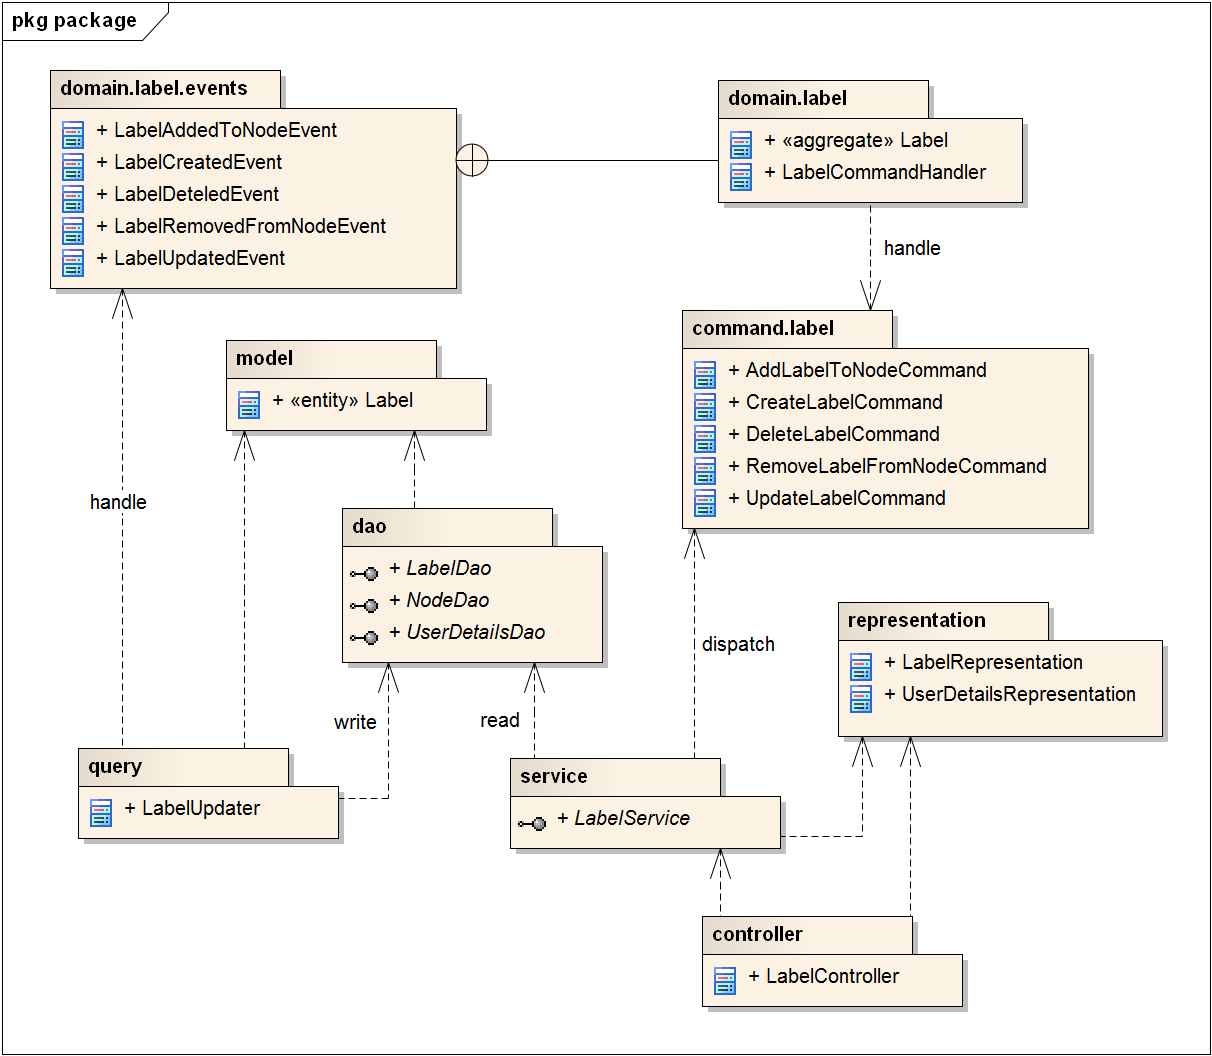
\includegraphics[width=0.98\columnwidth]{figures/package/package}
\caption{Overview of package structure for label functionality%
}
\end{center}
\end{figure}

The presented way of refactoring was applied similarly to other aspects
of the original domain model. This resulted in a number of new
aggregates that use event sourcing as their backing repository to take
care of business logic and upholding the invariants. Event processing
then ensured that the read model is built accordingly.


\subsubsection{User management}\label{user-management}

A small portion of the application was subjected to more than
refactoring to improve the user experience with the system. The portion
was related to user management, specifically registration and password
restoration. The original code didn't provide a great experience for
that functionality --- the registration of externs had to be done by
administrators that had to set up users including the passwords which
must have been sent by e-mail (or other means) to each person manually.
This way was unreliable and put more weight on the administrators, it
also undermined security as the passwords were known to the
administrators sending them to the users. Sagas were a perfect fit to
redesign this portion of the system.

The first part, the registration process, in which a new user is created
in the system, was flawed by the missing e-mail address in the entity of
the user. Thus, the password could not be sent automatically to the
user. Usually, an e-mail address is crucial for user verification and
password restoration. So, the implementation was altered and the user
e-mail address must be included when registering a new user. If the
command succeeds and the new user is created, the user needs to verify
their e-mail address to set up a password. A saga that listens for the
\texttt{UserCreatedEvent} manages this business transactions and waits
for the user to verify their e-mail address. The whole process of the
saga is defined by the following steps:

\begin{enumerate}
\def\labelenumi{\arabic{enumi}.}
\tightlist
\item
  A user with an e-mail address is created in the state of needed e-mail
  verification.
\item
  The event starts a saga that creates a new random registration token
  for the user. This token is sent to the user's e-mail address.
\item
  Using an event scheduler, an event is scheduled which expires the
  token in one hour.
\item
  Following that:

  \begin{enumerate}
  \def\labelenumii{\alph{enumii})}
  \tightlist
  \item
    the user sets their password by using the token before it expires.
    The registration is complete and the user is verified; or
  \item
    the expire event is published and the token is invalidated. The user
    needs to request a new registration token to be able to set the
    password.
  \end{enumerate}
\end{enumerate}

Password restoration was designed similarly. When users forget their
password, the e-mail address is the only trusted communication channel
(since the verification above) to handle the restoration, i.e.~setting a
new password. To manage that process, a different saga, which follows
the steps below, is created:

\begin{enumerate}
\def\labelenumi{\arabic{enumi}.}
\tightlist
\item
  A user requests restoration of forgotten password in the UI.
\item
  The saga is started and a new random restoration token is created for
  the user. This token is sent to the user's e-mail address.
\item
  Using an event scheduler, an event is scheduled which expires the
  token in one hour.
\item
  Following that:

  \begin{enumerate}
  \def\labelenumii{\alph{enumii})}
  \tightlist
  \item
    the user sets their password by using the token, before it expires.
    The restoration is complete and the user can log in; or
  \item
    the expire event is published and the token is invalidated. The user
    needs to request a new restoration token to be able to set the
    password.
  \end{enumerate}
\end{enumerate}

As it turned out, the two processes were so similar, that the sagas
could share a great portion of the code in a common base class,
\texttt{AbstractExpirableUserTokenSaga}. The specialized classes for
each saga --- \texttt{UserEmailVerificationSaga}, and
\texttt{RestoreLostUserPasswordSaga} --- differ in only the types of the
events they listen to or schedule.

Even though the implementation of the sagas to support both of these
processes is ready, the functionality is put on hold until the mail
server and the corresponding infrastructure to send automated e-mails is
provided.


\subsection{Problem solving}\label{problem-solving}

A few problems arose in the process of refactoring caused by the
different approach that CQRS takes. The following lines describe the
problems and the steps taken to solving them.

\subsubsection{Dealing with consistency
issues}\label{dealing-with-consistency-issues}

One problem was encountered when designing the file system in the new
domain model, i.e.~the files and folders structure and its behavior. In
the original design, the file system model was achieved by the
\texttt{File} and \texttt{Folder} Hibernate entities that referenced
other entities of the same type to form a tree of relationships. These
entities were supposed to be refactored as well.

By the definition, an aggregate is a set of related objects that
represents a transaction boundary. This was considered in the
refactoring of the entities. There are some business rules that had to
be preserved when designing aggregates for the file system. The first
one is the consistency of the delete operation on a folder, the second
is the uniqueness of node name in a folder. These business rules could
be upheld by modeling the file system as one big aggregate, containing
folders and files in a tree hierarchy. However, the folders can be
nested, and so the aggregate could grow very large. Loading such an
aggregate with possibly thousands of objects would be incredibly
resource-intensive and impossible to scale. In
\cite{aggregate1}\cite{aggregate2}\cite{aggregate3} it is advised to
make aggregates small. Also, it provides some solutions to consistency
issues. So the folders and files were designed as self-contained
aggregates. Similarly to the original entities, the two new aggregates,
\texttt{Folder} and \texttt{File}, share some common functionality that
was abstracted to a parent class (\texttt{AbstractNodeAggregateRoot}).

\paragraph{Node name uniqueness}\label{node-name-uniqueness}

As the individual instances of the \texttt{Folder} aggregate have no
access to the names of the contained files and subfolders, it was needed
to find another way how to ensure uniqueness of node names in a folder.
To resolve this issue, a special read model is built by events to store
only identifiers of nodes and their names and parent folders. This model
is queried just before creating a new child node, renaming a node, or
moving a node to other folder to ensure uniqueness of the node name in
that particular folder. The read model is kept in sync accordingly with
the changes made to the nodes. There is no consistency issue here,
because building the read model, in this case, happens in the same
transaction as persisting changes of an aggregate instance.

\paragraph{Folder deletion}\label{folder-deletion}

The other problem was the delete operation on a folder. In the original
design, when a folder was deleted, it recursively deleted all the child
folders and files in one transaction via Hibernate's support of
collections. Now, that a folder is represented as an aggregate which
doesn't hold references to other child folders or files, it wasn't so
straightforward to recursively delete child nodes. This issue was not
easy to solve without a lot of experience with CQRS design. However, it
then occurred that a saga (or in this case, a process manager) could be
of use. This idea was validated by CQRS practitioners in
\cite{deleting}.

The basic principle is that the process manager (called
\texttt{FolderDeletionSaga} in the code) coordinates the deletion of
multiple aggregate instances representing the child nodes of a folder.
It is started by publishing event \texttt{FolderDeletionStartedEvent} by
the \texttt{Folder} aggregate instance, which marks the beginning of the
deletion process. Using the same consistent read model as above, it
initially queries for the children of the folder to delete. For each
child node (folder or file) it sends a new command to the respective
aggregate instance to delete itself first. File aggregate instances are
deleted trivially. For each child folder, however, a new process manager
is recursively instantiated to manage the deletion process of that
folder. When all the nodes are deleted from a folder, i.e.~the folder is
empty, the saga managing the folder deletion sends one final internal
command to the folder aggregate instance to mark it deleted. When the
top saga instance, that initiated the recursive deletion process, is
reached, the process is finished. Because the sagas are driven by events
published by the aggregates, it is very easy to track the state of the
deletion process.

\subsubsection{Privacy issues}\label{privacy-issues}

In Integration Portal, the system is prevented from unauthorized access
by requiring authentication. To successfully authenticate, a user needs
to provide the correct username (e-mail address in new user management)
and password. In return, an access token is sent to the client, which
needs be specified in every subsequent request. Users' passwords should
be handled very carefully, if anybody breaks into the application
database, they must not be able to get the raw passwords. Usually,
passwords are not stored in the database directly, but rather they are
hashed.

Because Event Sourcing instructs to save state changes as events to
persistent storage, this should also be applied when setting or changing
a users' passwords. However, events that store passwords should be
considered a privacy (and security) issue, even though the passwords are
hashed. If the event store database is compromised, all the events about
setting the users' passwords could be in risk of exploitation, including
the old users' passwords that changed in the past. For this reason,
events do not store passwords (or their hash codes) at all, and so
passwords are excluded from the event-sourced state. A hashed password
is saved into the read-side database in a command handler, outside of
aggregates or event handlers. A domain event notifying about a password
change still exists, but it does not carry password data in any form.

This exception has an impact on almost all the benefits that Event
Sourcing provides, but it is crucial for user privacy and security. On
the other hand, let's note that passwords are not needed for any other
purpose than authentication in most cases. This situation was a great
example of when Event Sourcing is unnecessary for some parts of a
system. It is fundamental to point out again, that the Event Sourcing
pattern, as well as any other, is not all or nothing and should be used
in appropriate places only.


\subsection{Testing}\label{testing}

As stated in the description of the refactoring strategy, the whole
process was continually validated by tests written using the test-driven
development methodology. The strategy was to write the tests first and
then perform refactoring on the code to make the tests pass. As the
refactoring was gradual, one domain entity at the time, the particular
tests were written before each part of the refactoring.

Although, the tests were written from scratch, they were based on the
scenarios found in the integration tests for the original Integration
Portal code. The tests followed the following scheme --- set up the
initial state for the test, dispatch a command, whose processing was
under test, and finally assert the correct state of the database (of the
read model effectively). Listing~\ref{lst:test} shows an
example of one of the tests. The tests were written in the Groovy
programming language \cite{groovy} by using Spock library \cite{spock},
a testing and specification framework.

\begin{lstlisting}[caption={An example of a test specification using Spock.
The first method tests successful creation of a new label.
The second method tests that creating a duplicate label throws an exception.},label={lst:test},captionpos=b,float,floatplacement=H]
public class CreateLabelIntegrationSpec 
        extends AbstractIntegrationSpecification {

    def "should create a label"() {
        when:
            dispatch new CreateLabelCommand(LabelId.of("1"), "work", "red")

        then:
            def label = get(Label, "1")
            label.id == "1"
            label.name == "work"
            label.color == "red"
            label.owner.id == "1"
    }

    def "creating duplicate label results in error"() {
        when:
            dispatch new CreateLabelCommand(LabelId.of("1"), "work", "red")
            dispatch new CreateLabelCommand(LabelId.of("2"), "work", "red")

        then:
            thrown(AlreadyExistsException)
    }

}
\end{lstlisting}

As you can see, the tests are easy to navigate by leveraging Groovy's
named blocks that refer to the BDD-style (Behavior Driver Development)
of writing tests, which is a feature of Spock Framework. A test method
usually follows the given-when-then paradigm, where the \texttt{given}
block sets up the environment for the test, the \texttt{when} block
executes the code under test, and the \texttt{then} block validates the
test assertions.

All the integration tests written for the refactoring follow the same
scheme:

\begin{enumerate}
\def\labelenumi{\arabic{enumi}.}
\tightlist
\item
  Optionally, set up the environment of the test scenario by dispatching
  commands
\item
  Dispatch the command(s) under test
\item
  Assert that

  \begin{enumerate}
  \def\labelenumii{\alph{enumii})}
  \tightlist
  \item
    the state of the database is correct by querying the Hibernate
    entity manager, or
  \item
    an expected exception is thrown
  \end{enumerate}
\end{enumerate}

The \texttt{dispatch()} method is a convenience method to send commands
to the command gateway in a test. The command gateway and the command
bus then processes the commands by executing a command handler as usual.
If new events are published by handling the commands, they are processed
by event listeners and the read model is built accordingly. Finally, the
tests assert the state of the database by querying the Hibernate entity
manager and checking the attribute values in the entities. In some
cases, like in the Listing~\ref{lst:test}, it is needed to assert that an
expected exception was thrown.

The code under test uses Hibernate to access the database in a uniform
way, regardless of the database type. For the test environment, an
embedded in-memory HSQL database is used to save resources and make the
tests run faster. Setting up the in-memory database is just a matter of
configuration of the test environment.


\subsection{Summary}\label{summary}

In this chapter, refactoring of Integration Portal application to CQRS
and Event Sourcing was described. This section summarizes the outcome of
the refactoring and presents suggestions for future work.

The system was originally written in a strict n-layered architecture,
where domain entities backed by Hibernate served the purpose of both
writing and reading. Both responsibilities were mixed together in the
service layer. Refactoring to CQRS lead to reducing the complexity by
designating the business and write logic to a different model, written
in Axon Framework. Using this framework, the responsibility of the write
model was to handle state changes (mainly by using Event Sourcing) and
the read model was built by the events published in the process of
changing state. To simplify the refactoring, the read model was
preserved in the original design.

Let's now describe a few benefits, which were brought by the refactored
version, as well as a few disadvantages. Furthermore, let's outline some
ways how to leverage this design for the next development of Integration
Portal.

\subsubsection{Benefits}\label{benefits}

Most of the benefits of the CQRS and ES designs that were described in
\ref{event-sourcing-and-cqrs-design-patterns}
\nameref{event-sourcing-and-cqrs-design-patterns} were not fully
leveraged after refactoring. The reason is that these patterns are
so-called enabling patterns. That means they give the developers more
options and tools to extend the functionality of the application in the
future. New possible features that are based on the new design will be
presented further in the text. For now, let's described the immediate
benefits brought by the refactoring in the following paragraphs.

\paragraph{Reduced code complexity}\label{reduced-code-complexity}

The code that provides access to state transitions, business logic, as
well as querying for data is centered in the service layer. The
implementation of the service layer before the refactoring, however, was
complex and hard to maintain. The dependencies and responsibilities of
the individual service classes were not clear. The code of the methods
usually mixed validation and business logic to update and query entities
at the same time.

The refactoring, that followed the presented strategy, didn't bring
clear read-write separation of the service layer to separate modules, as
the general CQRS pattern recommends, but it greatly simplified the
complexity of the service layer. Methods in the service layer now have
only one responsibility --- to query the read model or to send a command
to the write model. The query methods simply delegate queries to the DAO
layer, whereas the command methods create a command with data and the
target aggregate identifier and send it to the command gateway. The
responsibilities and the dependencies are now visible and clear.
Additionally, by implementing the CQRS in Axon Framework, the write
model, and the business logic is now more transparent and focused in one
place --- the aggregates, whose changes are triggered by command
handlers. On the other side, updates to the entities of the read model
are put in separate classes, whose methods are triggered by event
handlers when the state changes.

The responsibilities are now clearly divided into separate submodules.
More importantly, the coupling of the responsibilities is seamless
thanks to Axon Framework infrastructure, making it easier to maintain
and test. Because all the modules now have an explicit purpose, it is
easier to reason about extending the code with new features in the sense
of dividing responsibilities.

Even though the complexity and code entanglement at the lowest level was
reduced by the refactoring, the code got more complex from the
architecture point of view.

\paragraph{Commands and Events}\label{commands-and-events}

Representing commands and events in the form of classes makes it easy
for the developers to orient themselves in the use cases of the system.
Each command carries a clear intent about what should happen in the
domain, and each event distinctly announces to the listeners what
actually happened, so they can appropriately respond.

Furthermore, commands can be intercepted to be enriched or changed
before they are actually processed. For example, it was possible for the
commands to be assigned a currently logged-in user required by the
domain. This operation was dedicated to a single class and reused
seamlessly for many commands. In the original code, this wasn't
possible, and the code to query for the logged-in user needed to be
duplicated.

\paragraph{Old issues resolved}\label{old-issues-resolved}

One of the business rules of the simulated file system is that two nodes
(folders and files) must not have the same name under the same folder.
Before the refactoring, there was an issue with this rule, where nodes
could have the same name if they were located in the root of the file
system. This bug was caused by the mechanism chosen to guard this
uniqueness. The mechanism was a unique database index on the
\texttt{name} and \texttt{parent} columns, where the parent was a
foreign key reference to a folder entity. The problem was that when the
parent was \texttt{null} (marking the root of the file system tree), the
index didn't work. In the file system root, the node names could be
duplicated.

Because CQRS handles denormalized data in the read model very well, a
special table (and an entity) was created only to capture dependencies
of nodes and their names without any other node properties. This table
was queried to check if a name of some node is unique before any change
regarding the name uniqueness. The table was intentionally kept very
simple, so it does not use many resources when querying. More about the
node name uniqueness rule was presented in
\ref{dealing-with-consistency-issues}
\nameref{dealing-with-consistency-issues}.

Following the refactoring, changes in the user management were easier to
implement in the new design. Sagas and scheduled events are in the
center of user registration, verification, and initial password set up,
as well as restoration of forgotten password. By using Axon's sagas,
these long-running business transactions were easy to implement.

\paragraph{Testing}\label{testing}

Integration testing was simplified to only sending appropriate commands
and asserting the state of the database. It is worth to mention that
both the tests and the actual implementation use the same commands to
get the system to a specific state. Ultimately, this means that the
tests are driven by the use cases represented as a series of commands.
This way, we can design our tests according to domain-specific rules and
operations.

On top of that, by using CQRS and especially Event Sourcing, it is
possible to express tests purely in terms of commands and events when
testing aggregates in a domain. Since the input to an aggregate is a
command and state transition of an aggregate is always an event, the
complete test scenario can be defined using just these objects. They
usually follow the scheme of:

\begin{itemize}
\tightlist
\item
  given certain events in the past
\item
  when this commands executes
\item
  expect some events to be published
\end{itemize}

The tests written this way are expressive and clear in their intentions.
They can be viewed as a part of unit testing; however, since they are
mainly driven by functional requirements, they hardly depend on any
implementation details, making them less vulnerable to code changes
inside the aggregates.


\subsubsection{Disadvantages}\label{disadvantages}

As with every existing design choices, CQRS and Event Sourcing has
definitely some disadvantages too. In the following text, the
description of those that occurred in the refactoring is presented.

\paragraph{Steep learning curve}\label{steep-learning-curve}

The CQRS design pattern with Event Sourcing implemented using
Domain-Driven Design methodology and terminology is a lot to process for
a developer. It takes a lot of practice and experience to know what is
right and what is wrong for the application. For newcomers, it is very
hard to grasp all the essential aspects of the design, and, more
importantly, to use it well. In businesses, this steep learning curve
can play a major role in deciding whether to use this design or go the
traditional way.

\paragraph{Code explosion}\label{code-explosion}

In the original design, there were only interfaces that defined methods
of the service layer, and then the implementation that used entities to
do business logic and querying. Using Axon's way of implementing CQRS,
there was considerably more code to create and maintain. For every
command method before, there is now a new command class. For each
original entity, there is now an aggregate that the commands target. And
for each state change in the aggregates, there is an event class.

All these classes created in the refactoring are contained in close to
120 new files! This adds more complexity to the structure of Integration
Portal and makes it harder for developers to orient themselves in the
project. Although, majority of these classes are commands and events,
which are usually very small data holders. The remaining files contain
only the CQRS-specific classes --- command handlers, aggregates, value
objects, sagas, and read model updaters.

\paragraph{Code navigation}\label{code-navigation}

Axon Framework implements CQRS using the standard Java language
constructs. That means, that all the features your IDE provides for
development in Java work here as well. Most of the popular IDEs know how
to navigate their users to declarations and code usages, e.g.~methods,
fields or classes. However, the way how the code is decoupled by Axon
Framework makes it significantly harder to use these features. The
problem is caused by the nature of commands and events being passed
around without specifying a direct connection to methods for their
publishing or handling. For example, to find a handler method for a
command or event, developers need to search for an annotated method with
an argument of the same type as the command or event. This way is not
very convenient, nor fast for the developers.

The authors of Axon Framework knew about this annoyance, so they've
created a plugin \cite{idea-plugin} for IntelliJ IDEA, a Java IDE. The
plugin makes navigation to and from handler methods easier. Sometimes,
however, it is not fully reliable and stops working, from my experience.


\subsubsection{Suggestions}\label{suggestions}

As stated above, the design patterns are not easy to master in a short
notice. Since this was the first time I used the presented design
patterns in a project, not everything turned out to be good after
refactoring. In the following paragraphs, a few corrections and
improvements are suggested for the future development.

\paragraph{Create multiple bounded
contexts}\label{create-multiple-bounded-contexts}

During the refactoring, the importance of bounded contexts, a way of
separating unrelated responsibilities in the domain was underestimated.
In the end, it turned out that the system is actually made of smaller
domain models that could be separated. This also includes the aggregates
which can be broken into smaller consistency boundaries that relate to
different contexts. As Domain-Driven Design \cite{ddd} teaches us, the
domain model should be incrementally improved as our knowledge about the
domain increases.

The following list suggests an idea of how to break the current domain
model into smaller bounded contexts.

\begin{itemize}
\tightlist
\item
  \textbf{File system bounded context} -- all the aggregates that are
  part of the simulated file system can be placed here

  \begin{itemize}
  \tightlist
  \item
    Files
  \item
    Folders
  \item
    Users (in the sense of an owner of the nodes)
  \end{itemize}
\item
  \textbf{User management bounded context} -- the processes dealing with
  user management

  \begin{itemize}
  \tightlist
  \item
    Registration
  \item
    Forgotten password
  \end{itemize}
\item
  \textbf{Administration bounded context} -- the domain of system
  administration by super users

  \begin{itemize}
  \tightlist
  \item
    Organizational Units and their quotas
  \item
    User roles
  \item
    User administration
  \end{itemize}
\item
  \textbf{User settings bounded context} -- everything that can be set
  by a user

  \begin{itemize}
  \tightlist
  \item
    Labels
  \item
    User groups
  \end{itemize}
\end{itemize}

\paragraph{Do not force CQRS and Event
Sourcing}\label{do-not-force-cqrs-and-event-sourcing}

As stated multiple times in the previous text, CQRS and Event Sourcing
are not all or nothing design patterns. In some cases or some bounded
contexts, they cause more harm than good. Take for example, the user
password management --- users' old passwords (their hash values) should
not be stored in the event log because it creates a major privacy and
security risk. This is where Event Sourcing is not very beneficial.

As stated in the paragraphs about bounded contexts above, the user
password management could be placed into a different aggregate, which is
not event-sourced. Thus, user details could still be event-sourced, but
the user password would not.

In some bounded contexts, where a domain model is trivial, a simple CRUD
system could be used instead of forcing CQRS, e.g.~in the administration
bounded context. This technique was used in \cite{journey}. Note that
all the changes still need to be validated against the domain knowledge,
if it is truly inappropriate to use CQRS or ES. Investigate all the
benefits and disadvantages that arise from not using the patterns before
refactoring.

\paragraph{Denormalize read models}\label{denormalize-read-models}

The strategy of the refactoring was to preserve the original relational
database model, which would be used for querying. For now, the database
doesn't cause any problems. If the database or the particular model does
not suffice in the future, it is possible to create denormalized data
from the domain events to incorporate different read models or database
engines, e.g.~MongoDB (a document database). In any case, the CQRS and
ES enable the system to grow and scale in an optimized way.

\paragraph{Snapshotting}\label{snapshotting}

Event sourcing is now used in all the aggregates without snapshotting.
If system writes (i.e.~command processing) become slow, it may be caused
by too many events being queried and handled to get the aggregate
instance to the desired state before handling the state change.
According to Greg Young, the author of Event Sourcing, aggregates do not
need snapshotting if the number of events of an instance is in hundreds
\cite{greg-youtube}. If the number of events increases to thousands,
snapshotting is a good way to optimize the write model. For more
information about snapshotting in Axon Framework, see the Axon
documentation \cite{axon-docs}.

\paragraph{Specialized event store}\label{specialized-event-store}

Events are now stored in the same database as the read model --- a
PostreSQL database. This may not be a great choice for an event store
because it is not optimized to do this task, and what's more, it is
harder to implement publish-subscribe event processing on top of it. My
recommendation is to search for a different database engine to store the
events to. Particularly, EventStore \cite{eventstore} and Apache Kafka
\cite{kafka} seem to be great candidates as they refer to Event Sourcing
and processing in their overview and documentation.


\subsubsection{Future development}\label{future-development}

To build further upon the system featuring CQRS and Event Sourcing, a
few ideas for the future developers are presented below to explore.

\paragraph{Axon 3}\label{axon-3}

Version 3 of Axon Framework is under development targeting a release
date in the first quarter of 2016 \cite{axon}. It brings a refined way
of writing classes of aggregates and sagas, so they do not extend any
Axon's classes making the domain model clean of implementation details.
It also brings other interesting features such as scheduled commands and
aggregates being able to create other aggregate instances. All these new
features could be beneficial to the Integration Portal.

\paragraph{Separation to modules}\label{separation-to-modules}

As the code written in Axon Framework is nicely decoupled, the project
could be broken into smaller modules, each dealing with some specific
subdomain. Possibly, each bounded context could be separated to an
individual submodule. This approach can be further evolved into
microservices and better scalability.

\paragraph{Notifications}\label{notifications}

For better user experience on the front-end side of Integration Portal,
a notification system based on event handlers could be developed.
Notifications about various events relevant to users could be stored in
the database and shown when users open Integration Portal in their
browsers. On top of that, a real-time push notifications from the server
to the client can be achieved by using WebSockets or ServiceWorkers. The
same principle could be used to send notifications through e-mail
messages.

\paragraph{History of file/folder
changes}\label{history-of-filefolder-changes}

One feature that was planned from the beginning of the development of
Integration Portal was to support a history of changes made to a file or
a folder. This log would include information what was done to a node and
by who. More importantly, files should provide a list of all the
versions of the file data and a way to restore the old versions.

Because all the events about changes in node aggregates are now stored,
it is possible to read these events and build a read model to support
this kind of a history log. This, however, does not apply to restoring
back a specific version of a file, because the events do not contain the
data about the content. The reason is that the events would become too
large and would decrease the system performance significantly. One
workaround would be to store the data in another storage, and events
would refer to it by the aggregate identifier and a version, for
example.


\section{Comparison to traditional layered
architecture}\label{comparison-to-traditional-layered-architecture}

This last chapter before concluding the diploma thesis compares the
presented design patterns to the traditional layered architecture. The
reason why this architecture figures in the comparison is not
accidental. Not only is it used in Integration Portal, but also it's the
most used architectural pattern in Java enterprise applications
\cite{oreilly}. I've used this architecture myself for years in the
university and at work.

CQRS takes the main role in the comparison since it represents the most
radical changes in the design. However, event sourcing, even though it
is just an extension of CQRS write model, will be in focus too as it
affects other design choices of application.

Before getting into details, let's first settle what the term layered
architecture means. After that, some of the problems with that
architecture are presented followed by the comparison with CQRS and
Event Sourcing.

\subsection{Layered architecture}\label{layered-architecture}

Layered, or more commonly N-layer or layers, architecture is a pattern
that helps to structure applications to logical layers, each one being
at a particular level of an abstraction \cite{pattern-oriented}. The
benefit of this pattern is that the low- and high-level issues are
decoupled from each other, usually by some clean interface. The
communication is then achieved from high-level layers to the low-level
and back. By isolating components into layers, responsibilities should
not be mixed together, and changes in one layer should not affect other
layers.

It is the most common architecture pattern and the de facto standard for
most Java enterprise applications \cite{oreilly}. As such, the pattern
is carried out in one specific way in most JEE applications, although,
it is still valid by the general definition above. Conceptually, there
is nothing wrong with the general pattern, and it is still a good
practice in software development. However, there are some downsides in
the typical implementation of the pattern in JEE applications. Let's
describe the specific implementation in that environment.

Applications are usually composed of some components. The aim of the
layered architecture is to organize these components in horizontal
layers, each layer having a specific role and responsibility. In a
typical JEE application, according to \cite{javadocs}, there are three
layers:

\begin{itemize}
\tightlist
\item
  \textbf{presentation layer} -- user interface and browser
  communication
\item
  \textbf{service / business layer} -- business rules and functions
\item
  \textbf{data access layer} -- an abstraction of database reads and
  writes
\end{itemize}

Presentation layer, for example, has just one responsibility --- display
the information to a user. It does not need to know anything about how
the data is stored. This is a responsibility of the data access layer.

On top of that, some kind of Object-Relational Mapping (ORM) is involved
in the data access layer that maps the data in a relational database
(rows of tables) into Java objects called entities or entity beans.
These objects are then passed between the other layers to execute
business logic on the data or to present the data to a client. Many
implementations of the pattern map the ORM entities to other objects ---
domain entities, data transfer objects --- which are used in
communication between two layers. This helps to define a strict
interface between the layers. Figure~\ref{fig:layered1} shows how the
layers are stacked and how they communicate. The strict separation by
interfaces makes the layers more decoupled and less prone to changes in
other layers. Also, implementation of the components can be completely
replaced without the interface being changed.


\begin{figure}[h!]
\begin{center}
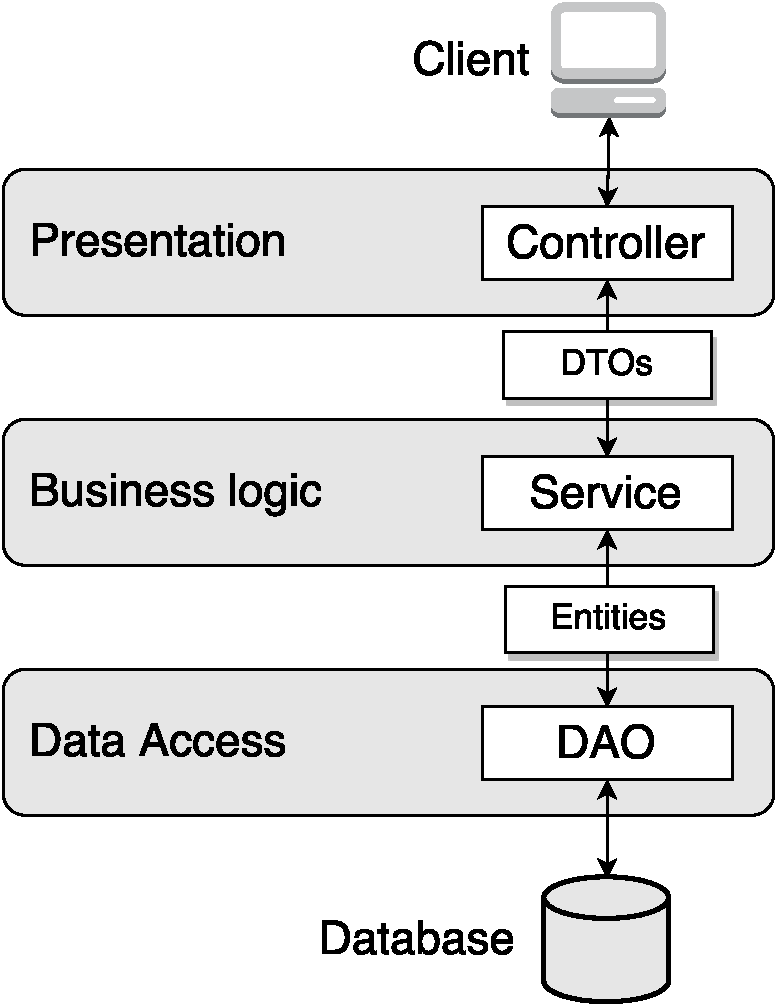
\includegraphics[width=0.42\columnwidth]{figures/layered1/layered1}
\caption{Common layers in enterprise applications%
}
\end{center}
\end{figure}

\subsubsection{Disadvantages}\label{disadvantages}

The layered architecture is the most common architecture pattern for
valid reasons because mixing low-level (e.g.~data persistence, web
services) and high-level (e.g.~presentation, business logic) makes the
code error-prone, harder to navigate, maintain and test. In general, it
is a good practice to follow this pattern. However, that doesn't mean it
has no disadvantages. Let's describe some of the problems of this
pattern in the following text.

\paragraph{Violation of single responsibility
principle}\label{violation-of-single-responsibility-principle}

Strict communication between stacked layers results in a situation where
the business layer has to be accessed to only query data. This violates
the single responsibility principle \cite{srp-violation}, that
encourages classes to have only one responsibility, one reason to
change. Responsibilities for validation and execution of user actions,
as well as queries, permeate into both data access and business logic
layers.

\paragraph{Leaky abstraction}\label{leaky-abstraction}

We can look at layers as abstractions of implementation details. For
example, presentation layer does not need to know how business logic is
handled or where and how the data is stored. However, \emph{all
non-trivial abstractions, to some degree, are leaky}, as the law of
leaky abstractions says \cite{leaky}. This leakage also affects the
layered architecture. Often, there are many abstractions in sequence
below presentation layer, e.g.~business layer, data access layer, remote
call, ORM, SQL. All these abstractions tend to leak in some way which
affects the upper layers. This can influence many aspects of the system,
such as performance and scalability.

\paragraph{Anemic model}\label{anemic-model}

The way how the layers are constructed encourages developers to create
anemic domain model \cite{layered-anemic}. That is a model where domain
entities contain little or no business logic and usually, just expose
getters and setters of their fields \cite{anemic}. Although anemic
entities follow single responsibility principle, as the only reason to
change them is when data structure changes, the business logic is
disconnected from the data. This goes against the basic principles of
object-oriented design, where objects combine data and operations
together to form one self-contained object that guards its invariants
and state.

Although, this model is justifiable in simple applications, such as
CRUD-based domain, it goes against best-practice principles of
encapsulation and information hiding. The logic is separated to a
business layer, possibly in a number of places making it hard to
maintain the code. Domain objects cannot guarantee their business rules
and invariants for themselves.

\paragraph{Layer-to-layer delegation}\label{layer-to-layer-delegation}

In very simple, mostly CRUD-based, applications, code written in
strictly layered design makes the components very thin with no added
value \cite{oreilly}. Implementations usually just delegate calls from
one layer to the other just to conform to the strict top-down way of
processing a request. When implementing a new feature, it usually means
to add unnecessary code to the project just for the sake of having
layers.

But, as written above, separating the responsibilities makes the code
less coupled. So these layers get more handy when changing
implementations, e.g.~when replacing the implementation of the data
source.

\paragraph{Tight coupling}\label{tight-coupling}

Even though, the layers (and their responsibilities) are decoupled from
each other, they usually, based on the underlying implementation, are
not loosely coupled \cite{oreilly}. Specifically, both presentation
layer and business layer depend on the data access layer. Thus, data
access logic is omnipresent in the code. This tends to make the system
monolithic, which in turn can pose some potential issues with
deployment, robustness, reliability, and scalability \cite{oreilly}.


\subsection{Effects of CQRS and ES on
architecture}\label{effects-of-cqrs-and-es-on-architecture}

To be accurate, neither CQRS nor ES are patterns that could supersede
the layered architecture (or any other), because they are very simple
principles in the core, and not architectural designs per se. With that
being said, layers are a good practice to hold to in any case. However,
CQRS and ES have a big effect on the traditional architecture and design
process.

\paragraph{Domain centric}\label{domain-centric}

One of the most visible changes is the focus of development. In the
traditional layered architecture, it is the database and structure of
the data that is in the center. The service layer with business logic is
then applied on top of it in a separate layer. In CQRS (written in DDD
style), the domain model is the core of development effort, usually
driven by use cases and problems in the domain. Of course, to act upon
the domain model, it still needs some data access layer to get aggregate
instances (or, in the case of ES, events), but the dependency is now
reversed. The business logic does not depend on the data access layer.
This has a number of benefits, e.g.~it makes it a lot easier to test the
business logic, and also it is not affected by leaky abstraction of the
data access layer.

This pushes the design more to the hexagonal \cite{hex} or clean
\cite{clean} architecture, which puts the domain and business logic into
the center. This also turns the domain away from the anemic model that
was often found in the traditional design.

\paragraph{Separation of concerns}\label{separation-of-concerns}

In the traditional layered architecture, a request for a query always
needs to go through the business layer to get to the data access layer,
even though it does not do anything business-specific and is free of
side effects. In CQRS, the domain is not bloated with presentation
issues, because the read model is built by event handlers with its own
data access objects completely outside of this layer. This reduces the
amount of code needed to implement queries and removes the pure
delegation of methods between layers.

\paragraph{Loose coupling}\label{loose-coupling}

Commands and events also greatly reduce coupling between layers. A
command represents a request for some task to be done, but it does not
depend on any concrete component that executes the task (except for the
command bus that dispatches the command). The same applies to events,
where event listeners are completely decoupled from publishers.

\paragraph{Scalability and
performance}\label{scalability-and-performance}

The clear separation of read and write models and the way the components
are decoupled opens the way to increase scalability and performance. It
is possible to easily include queues and messaging buses to the system
to provide partitioning of command and event processing using
asynchronous execution. This, in turn allows for scaling the read and
write models independently of each other. As stated in
\ref{command-query-responsibility-segregation}
\nameref{command-query-responsibility-segregation}, the read model can
be \emph{eventually consistent} and denormalized to views, which causes
the application to perform better.

\paragraph{Testability}\label{testability}

Layered architecture is testable, but it requires a lot of mocking and
set up, because of coupling. For example, business logic needs to mock
data access layer to instantiate and retrieve the domain objects
(entities) and then the tests asserts the state of entities being saved
back to the data access layer.

In CQRS, the components are nicely decoupled and driven by events and
commands. This makes unit testing far more easy. In the case of Event
Sourcing, where the domain events are the main source to build a state,
we can express test scenarios purely in terms of events.


\section{Conclusion}\label{conclusion}

This diploma thesis aimed at implementing the Event Sourcing and CQRS
design patterns in the Java programming language. Because these patterns
are not widely known in the Java world, they were briefly introduced to
the reader together with Domain-Driven Design methodology. These design
patterns were studied thoroughly, so they could be applied to a real
Java project --- Integration Portal. The refactoring of the system's
original design to CQRS and ES was achieved by using Axon Framework, a
Java library that supports software development by the principles of the
two patterns. The strategy and the process of the refactoring were
described, followed by solutions to some problems that were encountered.
Finally, the original layered architecture was described pointing out
its disadvantages, and compared to the new design. To conclude, the
following paragraphs evaluate the outcome of the thesis, particularly
the use of the two design patterns in Java and in general.

\subsection{Evaluation of CQRS and Event
Sourcing}\label{evaluation-of-cqrs-and-event-sourcing}

CQRS and Event Sourcing are definitely interesting patterns to further
explore. Not only they are empowering and enable a lot of possibilities
to developers, but they even improve the overall design and architecture
of an application. It reassured me of what I don't like about the
traditional layered architecture in enterprise applications.

A nice outcome of the refactoring was that the patterns didn't bring a
lot of breaking changes to the project. Although, the application of the
patterns usually results in bringing message queues, buses, and
asynchronous execution, which means a lot of work around the structure
and deployment of the application, this was not the case in the
refactoring. The application remained a monolithic, single module which
made the refactoring be a gradual improvement. But if the time comes for
the application to increase the scalability and availability, the CQRS
with Axon Framework enables that very easily by changing configuration
(and a bit of the code).

However, both of the patterns are not very easy to grasp. The steep
learning curve is the major disadvantage of the patterns and DDD, which
makes the adoption of the patterns in businesses difficult. There is a
lot to process for the developers and makes the structure of the
architecture more complex --- self-contained modules, asynchronous
execution, queues, etc. Also, they require that developers change their
mindset built by the traditional applications --- transaction scripts,
immediate availability and synchronous execution.

Overall, the patterns should get more of the popularity because they
enable a lot of possibilities (some described in
\ref{event-sourcing-and-cqrs-design-patterns}
\nameref{event-sourcing-and-cqrs-design-patterns}) and lead to better
domain-oriented, scalable and available applications. The path to that
is not easy, but it is rewarding at the end. Moreover, the clean and
hexagonal architectures, which are more convincing than the traditional
layered architecture, can be built on top of CQRS.

\subsection{Implementation in Java}\label{implementation-in-java}

In Java, the use of Axon Framework to implement the patterns was a good
decision, although there are some issues regarding implementation
details that the framework enforces to the code being developed. Some of
the downsides should be resolved in the next major version, which should
be released soon \cite{axon}. Even though the framework does not use the
now popular actor model and reactive programming that fit with the
paradigms, it is a solid, well-tested, integrable piece of a library
with many great features that makes the implementation of CQRS and ES
straightforward in Java.

On the other hand, Java is not a convenient language to implement CQRS
and ES, because the language is still very conservative about features
that could be beneficial in the development. Other languages, e.g.~C\#
or Scala, have a better support of making the code more maintainable and
easy to read. For Java, I decided to use Lombok library to diminish some
of the inconveniences.

\subsection{Integration Portal}\label{integration-portal}

I would recommend using the refactored version of Integration Portal
because it enables more flexibility than the original design. The
command- and event-based system definitely fits the domain and can be
leveraged in the integration of other systems. Querying the REST
interface could also be well optimized by using specialized read models
stored, for example, in a document database like MongoDB rather than the
rational database.

However, the biggest downside is that the Integration Portal team would
need to know these patterns well enough to expand the code. And as
stated previously, the learning curve is pretty steep and takes a lot of
time to learn CQRS and Event Sourcing (as well as the Domain-Driven
Design concepts), not to mention Axon framework. For these reasons, I
would recommend to continue on the refactored version to interested
people only. On the contrary, expanding the functionality of the
original design could backfire in the long term because of the mixed
concerns and code complexity, which will definitely rise if not taken
care of.

\subsection{Final thoughts}\label{final-thoughts}

Overall, I am satisfied with the outcome of this project. I expanded my
knowledge of design patterns that can help me make better applications.
My personal experience with the CQRS and Event Sourcing patterns was
very educational. Although, I may not use the patterns in every future
application, they certainly changed my mindset about the architecture
and structure of applications and that it is important to reason about
it in details.

The implementation of the patterns resulted in better and cleaner
architecture of the Integration Portal project, and also enabled new
possibilities to expand its functionality and to easily add new
features. However, there was a lot to learn to make it happen and there
was not enough time to incorporate the expanded CQRS design with
asynchronous execution and a number of optimized read models. This idea
is left for future work.

In conclusion, I found the patterns to be very interesting, and I will
definitely explore them more in the future.


\bibliography{bibliography/converted_to_latex.bib%
}

\end{document}

